\chapter{CSP Models for Puzzle Games}
\label{cha:design}
Generally, this chapter discusses two parts: the CSP model and its encodings for the 2D game (IQ Twist), the CSP models and their encodings for the two playing modes of the 3D game (Zig Zag Puzzler).
\section{IQ Twist}
IQ Twist is a puzzle game that consists of 8 twisted puzzle pieces and 7 coloured pegs (Figure~\ref{fig:IQ_twist_game}). To play the game, the colored pegs should be placed on the board in advance, then one has to fit all the twisted puzzle pieces back into the board. Different units of piece have to match the pegs with the same color and only the hollow units of a piece can be used to match pegs. Moreover, the difficulty of a single game depends on the pegs' placements given at the beginning.
\begin{figure}[htbp]
    \centering
    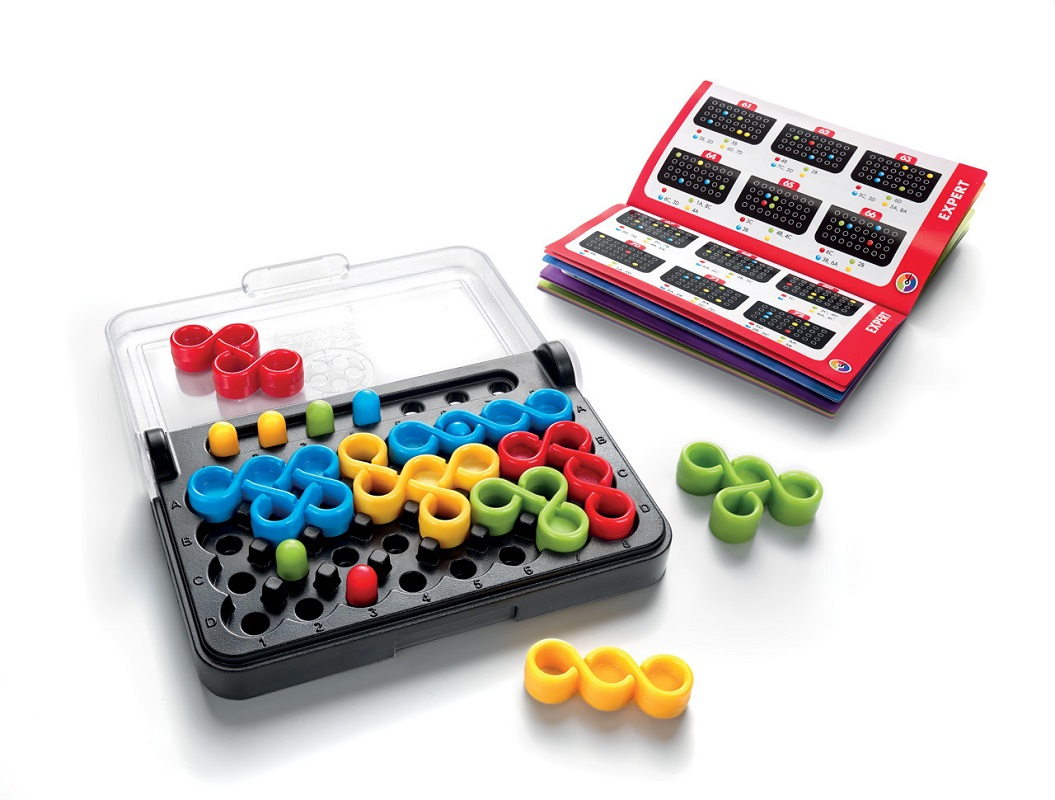
\includegraphics[width=0.6\textwidth]{figs/IQtwistintroduction.jpg}
    \caption{IQ Twist game, adopted from~\cite{r21}}
    \label{fig:IQ_twist_game}
\end{figure}
\subsection{Variables}
First of all, the initial state of each piece is defined in Figure~\ref{fig:allinit}.
\begin{figure}[htbp]
\begin{subfigure}[b]{.24\textwidth}
\centering

\includegraphics[width=0.75\textwidth]{figs/yellow1.jpg}
\caption{Initial state of yellow1}
  \label{fig:2Dyellow1}
\end{subfigure}
\begin{subfigure}[b]{.24\textwidth}
\centering
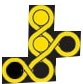
\includegraphics[width=0.75\textwidth]{figs/yellow2.jpg}
\caption{Initial state of yellow2}
  \label{fig:2Dyellow2}
\end{subfigure}
\begin{subfigure}[b]{.24\textwidth}
\centering
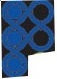
\includegraphics[width =0.5\textwidth]{figs/blue1.jpg}
\caption{Initial state of blue1}
  \label{fig:2Dblue1}
\end{subfigure}
\begin{subfigure}[b]{.24\textwidth}
\centering

\includegraphics[width=\textwidth]{figs/blue2.jpg}
\caption{Initial state of blue2}
  \label{fig:2Dblue2}
\end{subfigure}
\begin{subfigure}[b]{.24\textwidth}
\centering

\includegraphics[width=0.75\textwidth]{figs/green1.jpg}
\caption{Initial state of green1}
  \label{fig:2Dgreen1}
\end{subfigure}
\begin{subfigure}[b]{.24\textwidth}
\centering

\includegraphics[width =0.5\textwidth]{figs/green2.jpg}
\caption{Initial state of green2}
  \label{fig:2Dgreen2}
\end{subfigure}
\begin{subfigure}[b]{.24\textwidth}
\centering

\includegraphics[width =\textwidth]{figs/red1.jpg}
\caption{Initial state of red1}
  \label{fig:2Dred1}
\end{subfigure}
\begin{subfigure}[b]{.24\textwidth}
\centering

\includegraphics[width=0.75\textwidth]{figs/red2.jpg}
\caption{Initial state of red2}
  \label{fig:2Dred2}
\end{subfigure}
\caption{Initial state of each piece}
  \label{fig:allinit}
\end{figure}
There are some name rules. Firstly, all the variables are corresponding to the specific unit of a piece. As an example, for piece yellow2, Figure~\ref{fig:namerules} shows that the first variable $V_{y21}$ is used to represent the left-most bottom unit. For other units, they are named as $V_{y22}$, $V_{y23}$, $V_{y24}$ and $V_{y25}$, which follows the order from left to right and bottom-up. Similarly, the name rules will be used for other pieces. 
\begin{figure}[htbp]
    \centering
    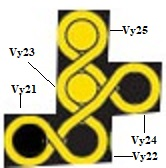
\includegraphics[width=0.3\textwidth]{figs/example.jpg}
    \caption{Name rules of yellow2}
    \label{fig:namerules}
\end{figure}
In addition, there are seven pegs. Each of them is assigned a variable, the subscript represents its color such as $V_{py1}$ that $_{py1}$ stands for yellow peg1. Therefore, the variables can be represented as $\VUnits$ and $\VPegs$,
\begin{equation}
\begin{aligned}
\VUnits=\{&V_{y11},V_{y12},V_{y13},\\&V_{y21},V_{y22},V_{y23},V_{y24},V_{y25},\\&V_{b11},V_{b12},V_{b13},V_{b14},
V_{b15},\\&V_{b21},V_{b22},V_{b23},V_{b24},\\&V_{g11},V_{g12},V_{g13},V_{g14},\\&V_{g21},V_{g22},V_{g23},\\&V_{r11},
V_{r12},V_{r13},V_{r14},\\&V_{r21},V_{r22},V_{r23},V_{r24}\},\\
\\\VPegs = \{&V_{py1}, V_{py2}, V_{pb1}, V_{pb2}, V_{pg1}, V_{pg2}, V_{pr}\},\\
\\V = &\VUnits \cup \VPegs.
\end{aligned}
\end{equation}
\subsection{Domain}
\begin{figure}[htbp]
\centering
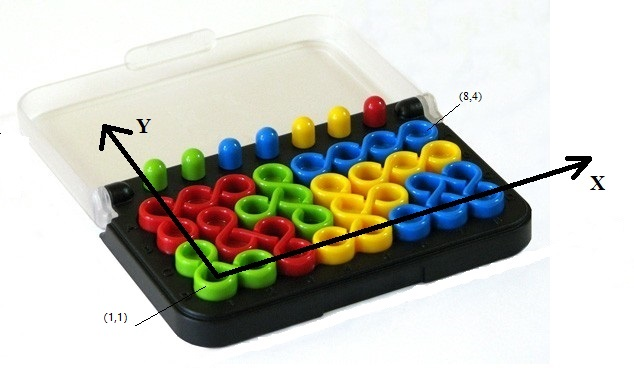
\includegraphics[width=0.6\textwidth]{figs/IQtwistboard.jpg}
\caption{The coordinate system for IQ Twist, revised from~\cite{r22}}
    \label{fig:coordinate}
\end{figure}
For the board, Figure~\ref{fig:coordinate} shows that the 2D coordinate system is used to describe the positions. In our model, all positions are represented as tuples and each tuple consists of 2 elements that are integers. The left-most bottom position is $(1,1)$ and the right and top is $(8,4)$. So, the abscissa for each unit of piece will be from 1 to 8 and the ordinate will be from 1 to 4. Considering a position $(x_{0},y_{0})$, we get
\begin{equation}
\begin{aligned}
&0<x_{0} \leq 8,\\
&0<y_{0} \leq 4.
\end{aligned}
\end{equation}
The placements for each unit of pieces must on the board, therefore, we get
\begin{equation}
\forall  v \in \VUnits \hspace{1ex},\hspace{1ex} D(v)=\{(i,j) \in \mathbb{N} \times \mathbb{N}	\mid  0<i \leq 8 \hspace{1ex} , \hspace{1ex} 0<j \leq 4\}.\\
\end{equation}
The pegs are special because they can be put in any places on the board or not on the board. So, the domain of pegs is
\begin{equation}
\forall  v \in \VPegs \hspace{1ex},\hspace{1ex} D(v)=\{(0,0)\} \hspace{1ex} \cup \hspace{1ex}\{(i,j) \in \mathbb{N} \times \mathbb{N}\mid  0<i \leq 8 \hspace{1ex} , \hspace{1ex} 0<j \leq 4\}.
\end{equation}
\subsection{2D Rotation Matrix}
\label{section:2Drotationmatrix}
To clarify how to obtain all configurations for each piece, the 2D rotation matrix will be introduced. 
\\In Figure~\ref{fig:explanation2D}, the unit which is corresponding to the first variable $V_{y21}$ can be considered as a point $(x_{0},y_{0})$. In a general case without the domain of IQ Twist, if we assign (0,0) to $(x_{0},y_{0})$, the $V_{y21}$, $V_{y22}$, $V_{y23}$, $V_{y24}$ and $V_{y25}$ can be respectively represented as $(0,0)$, $(1,0)$, $(1,1)$, $(2,1)$ and $(1,2)$, which indicate that all other variables are connected with the first variables. For example, if $x_{V}$ corresponds to the $x$ position of unit piece $V$ and $y_{V}$ corresponds to the $y$ position of unit piece $V$, there are relationships
\begin{equation}
\begin{aligned}
&x_{V_{y21}}+1=x_{V_{y22}},\\
&y_{V_{y21}}=y_{V_{y22}},
\end{aligned}
\end{equation}
between $V_{y21}$ and $V_{y22}$.
\begin{figure}[htbp]
\centering
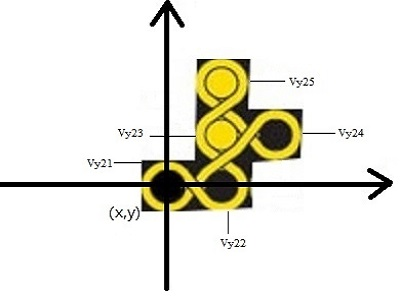
\includegraphics[width=0.5\textwidth]{figs/explanation2D.jpg}
\caption{Explanation of 2D rotation}
    \label{fig:explanation2D}
\end{figure}
Therefore, all other placements can be obtained from the initial state of the piece by rotations around the unit of piece $V_{y21}$.\\
Tobias and Krantz~\cite{r9} mention that 2D counterclockwise rotation by an angle $\theta$ around the origin of a coordinate can be described as a matrix
\begin{equation}
R(\theta)=\begin{bmatrix}
\cos\theta & -\sin\theta\\
\sin\theta & \cos\theta\\
\end{bmatrix}.
\end{equation}
If the initial position is (x,y), the position after the rotation can be obtained by
\begin{equation}
\label{equation:rotation}
\begin{bmatrix}
x'\\
y'\\
\end{bmatrix}
=\begin{bmatrix}
\cos\theta & -\sin\theta\\
\sin\theta & \cos\theta\\
\end{bmatrix}
\begin{bmatrix}
x\\
y\\
\end{bmatrix},
\end{equation}
which implies that 
\begin{equation}
\label{equation:formula1}
\begin{aligned}
&x'=x\cos\theta-y\sin\theta,\\
&y'=x\sin\theta+y\cos\theta.
\end{aligned}
\end{equation}
Therefore, if 0, 90, 180 and 270 degrees are assigned to $\theta$, there are four configurations:
\begin{enumerate}
  \item $x'=x\cos0^{\circ} - y\sin0^{\circ}\hspace{20pt},y'=x\sin0^{\circ} + y\cos0^{\circ}\hspace{24pt}\implies x'=x\hspace{10pt}, y'=y$
  \item $x'=x\cos90^{\circ} - y\sin90^{\circ}\hspace{10pt},y'=x\sin90^{\circ} + y\cos90^{\circ}\hspace{12pt}\implies x'=-y, y'=x$
  \item $x'=x\cos180^{\circ} - y\sin180^{\circ}, y'=x\sin180^{\circ} + y\cos180^{\circ} \implies x'=-x, y'=-y$
  \item $x'=x\cos270^{\circ} - y\sin270^{\circ}, y'=x\sin270^{\circ} + y\cos270^{\circ} \implies x'=y\hspace{10pt},y'=-x$
  \label{rotation4}
\end{enumerate}
In IQ Twist, there exists a mirroring operation which corresponds to flipping a piece, if a unit of piece flips over around the y-axis, we get  (-x,y) from (x,y). Similarly, all the four configurations flip over around the y-axis. We get four more configurations: 
\begin{enumerate}
\setcounter{enumi}{4}
  \item  $x'=x\hspace{10pt}, y'=y\hspace{10pt}$    flip over around the y-axis $\implies x''=-x\hspace{8pt},y''=y$
  \item  $x'=-y, y'=x\hspace{10pt}$                flip over around the y-axis $\implies x''=y,y''=x$
  \item  $x'=-x, y'=-y$               flip over around the y-axis $\implies x''=x, y''=-y$
  \item  $x'=y\hspace{10pt},y'=-x$    flip over around the y-axis $\implies x''=-y\hspace{8pt}, y''=-x$
  \label{mirrorrotate4}
\end{enumerate}
Therefore, there should be a total of eight configurations for each unit of piece.
As an instance, for all units of the piece in Figure~\ref{fig:explanation2D}, considering a general case where a coordinate system includes negative values, if we assign $(0,0)$ to $(x_{0},y_{0})$, the process of rotation for each other unit of the piece can be represented by Equation~\ref{equation:rotation}. Figure~\ref{fig:Exampleof8} shows the eight configurations of yellow2.
\begin{figure}[htbp]
\centering
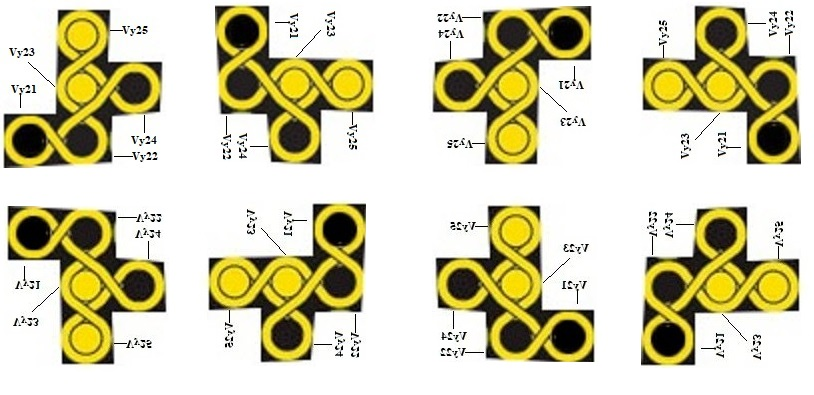
\includegraphics[width =\textwidth]{figs/domainexplain.jpg}
    \caption{Example of 8 configurations}
    \label{fig:Exampleof8}
\end{figure}
Accordingly, we get eight possible configurations
\begin{enumerate}
 \label{enu:eightsituation}
 \item $V_{y21}=(0,0)$, $V_{y22}=(1,0)$, $V_{y23}=(1,1)$, $V_{y24}=(2,1)$, $V_{y25}=(1,2)$,
 \item $V_{y21}=(0,0)$, $V_{y22}=(0,1)$, $V_{y23}=(-1,1)$, $V_{y24}=(-1,2)$, $V_{y25}=(-2,1)$,
 \item $V_{y21}=(0,0)$, $V_{y22}=(-1,0)$, $V_{y23}=(-1,-1)$, $V_{y24}=(-2,-1)$, $V_{y25}=(-1,-2)$,
 \item $V_{y21}=(0,0)$, $V_{y22}=(0,-1)$, $V_{y23}=(1,-1)$, $V_{y24}=(1,-2)$, $V_{y25}=(2,-1)$,
 \item $V_{y21}=(0,0)$, $V_{y22}=(-1,0)$, $V_{y23}=(-1,1)$, $V_{y24}=(-2,1)$, $V_{y25}=(-1,2)$,
 \item $V_{y21}=(0,0)$, $V_{y22}=(0,1)$, $V_{y23}=(1,1)$, $V_{y24}=(1,2)$, $V_{y25}=(2,1)$,
 \item $V_{y21}=(0,0)$, $V_{y22}=(1,0)$, $V_{y23}=(1,-1)$, $V_{y24}=(2,-1)$, $V_{y25}=(1,-2)$,
 \item $V_{y21}=(0,0)$, $V_{y22}=(-1,0)$, $V_{y23}=(-1,-1)$, $V_{y24}=(-2,-1)$, $V_{y25}=(-1,-2)$.
\end{enumerate}
Considering the domain of IQ Twist again, the piece can be moved as long as all units of the piece are on the board. Both $x_{0}$ and $y_{0}$ can be variables, hence we get the general forms 
\begin{enumerate}
 \label{enu:formuals}
 \item $V_{y21}=(x_{0},y_{0})$, $V_{y22}=(x_{0}+1,y_{0})$, $V_{y23}=(x_{0}+1,y_{0}+1)$, $V_{y24}=(x_{0}+2,y_{0}+1)$, $V_{y25}=(x_{0}+1,y_{0}+2)$,
 \item $V_{y21}=(x_{0},y_{0})$, $V_{y22}=(x_{0},y_{0}+1)$, $V_{y23}=(x_{0}-1,y_{0}+1)$, $V_{y24}=(x_{0}-1,y_{0}+2)$, $V_{y25}=(x_{0}-2,y_{0}+1)$,
 \item $V_{y21}=(x_{0},y_{0})$, $V_{y22}=(x_{0}-1,y_{0})$, $V_{y23}=(x_{0}-1,y_{0}-1)$, $V_{y24}=(x_{0}-2,y_{0}-1)$, $V_{y25}=(x_{0}-1,y_{0}-2)$,
 \item $V_{y21}=(x_{0},y_{0})$, $V_{y22}=(x_{0},y_{0}-1)$, $V_{y23}=(x_{0}+1,y_{0}-1)$, $V_{y24}=(x_{0}+1,y_{0}-2)$, $V_{y25}=(x_{0}+2,y_{0}-1)$,
 \item $V_{y21}=(x_{0},y_{0})$, $V_{y22}=(x_{0}-1,y_{0})$, $V_{y23}=(x_{0}-1,y_{0}+1)$, $V_{y24}=(x_{0}-2,y_{0}+1)$, $V_{y25}=(x_{0}-1,y_{0}+2)$,
 \item $V_{y21}=(x_{0},y_{0})$, $V_{y22}=(x_{0},y_{0}+1)$, $V_{y23}=(x_{0}+1,y_{0}+1)$, $V_{y24}=(x_{0}+1,y_{0}+2)$, $V_{y25}=(x_{0}+2,y_{0}+1)$,
 \item $V_{y21}=(x_{0},y_{0})$, $V_{y22}=(x_{0}+1,y_{0})$, $V_{y23}=(x_{0}+1,y_{0}-1)$, $V_{y24}=(x_{0}+2,y_{0}-1)$, $V_{y25}=(x_{0}+1,y_{0}-2)$,
 \item $V_{y21}=(x_{0},y_{0})$, $V_{y22}=(x_{0}-1,y_{0})$, $V_{y23}=(x_{0}-1,y_{0}-1)$, $V_{y24}=(x_{0}-2,y_{0}-1)$, $V_{y25}=(x_{0}-1,y_{0}-2)$,
\end{enumerate}
where the abscissa of each variable is from 1 to 8 and the ordinate of each variable is from 1 to 4.  
\subsection{Constraints}
\label{section:IQtwistconstriant}
Firstly, there should be no two different units of a piece take up the same position
\begin{equation}
\label{equ:firstconstrain}
\begin{aligned}
&\forall v_{m},v_{n} \in \VUnits\quad \text{where} \quad v_{m} \neq v_{n}:\\
&\Constraints{m}{n}=\{((x_{1},y_{1}),(x_{2},y_{2}))\in \Domain{m} \times \Domain{n}\mid x_{1} \neq x_{2}   \hspace{1ex} or \hspace{1ex}  y_{1} \neq y_{2}\}.
\end{aligned}
\end{equation}
Secondly, there should be no two different pegs that take up the same position except both of them are not on the board
\begin{equation}
\label{equ:secondconstrain}
\begin{aligned}
&\forall v_{m},v_{n}\in \VPegs \quad \text{where} \quad v_{m} \neq v_{n}:\\
&\Constraints{m}{n}=\{((x_{1},y_{1}),(x_{2},y_{2}))\in \Domain{m}\times \Domain{n}\mid x_{1} \neq x_{2}   \hspace{1ex} or \hspace{1ex}  y_{1} \neq y_{2}\}\hspace{1pt}\cup \\
&\{((0,0),(0,0))\}.
\end{aligned}
\end{equation}
As is mentioned in Chapter~\ref{section:2Drotationmatrix}, there should be eight configurations for the general pieces. Figure~\ref{fig:Exampleof8} shows the eight configurations for yellow2. Hence,
\begin{equation}
\label{equ:thirdconstrain}
\begin{aligned}
\Cons{y21}{y22}{y23}{y24}{y25}=\{&((x_{1},y_{1}),(x_{2},y_{2}),(x_{3},y_{3}),(x_{4},y_{4}),(x_{5},y_{5}))\in \\
&\Domain {y21} \times \Domain{y22}\times \Domain{y23}\times \Domain{y24}\times \Domain{y25} \mid\\
&(x_{2} = x_{1} + 1,\hspace{1ex}y_{2} = y_{1},\hspace{1ex}x_{3} = x_{1}+1,\hspace{1ex}y_{3} = y_{1}+1,
\\&x_{4} = x_{1}+2,\hspace{1ex}y_{4} = y_{1}+1,\hspace{1ex}x_{5} = x_{1}+1,\hspace{1ex}y_{5} = y_{1}+2)\hspace{1ex} or \\
&(x_{2} = x_{1} ,\hspace{1ex}y_{2} = y_{1}+1,\hspace{1ex}x_{3} = x_{1}-1,\hspace{1ex}y_{3} = y_{1}+1,
\\&x_{4} = x_{1}-1,\hspace{1ex}y_{4} = y_{1}+2,\hspace{1ex}x_{5} = x_{1}-2,\hspace{1ex}y_{5} = y_{1}+1)\hspace{1ex} or \\
&(x_{2} = x_{1}-1 ,\hspace{1ex}y_{2} = y_{1},\hspace{1ex}x_{3} = x_{1}-1,\hspace{1ex}y_{3} = y_{1}-1,
\\&x_{4} = x_{1}-2,\hspace{1ex}y_{4} = y_{1}-1,\hspace{1ex}x_{5} = x_{1}-1,\hspace{1ex}y_{5} = y_{1}-2)\hspace{1ex} or \\
&(x_{2} = x_{1} ,\hspace{1ex}y_{2} = y_{1}-1,\hspace{1ex}x_{3} = x_{1}+1,\hspace{1ex}y_{3} = y_{1}-1,
\\&x_{4} = x_{1}+1,\hspace{1ex}y_{4} = y_{1}-2,\hspace{1ex}x_{5} = x_{1}+2,\hspace{1ex}y_{5} = y_{1}-1)\hspace{1ex} or \\
&(x_{2} = x_{1}-1 ,\hspace{1ex}y_{2} = y_{1},\hspace{1ex}x_{3} = x_{1}-1,\hspace{1ex}y_{3} = y_{1}+1,
\\&x_{4} = x_{1}-2,\hspace{1ex}y_{4} = y_{1}+1,\hspace{1ex}x_{5} = x_{1}-1,\hspace{1ex}y_{5} = y_{1}+2)\hspace{1ex} or \\
&(x_{2} = x_{1} ,\hspace{1ex}y_{2} = y_{1}-1,\hspace{1ex}x_{3} = x_{1}-1,\hspace{1ex}y_{3} = y_{1}-1,
\\&x_{4} = x_{1}-1,\hspace{1ex}y_{4} = y_{1}-2,\hspace{1ex}x_{5} = x_{1}-2,\hspace{1ex}y_{5} = y_{1}-1)\hspace{1ex} or \\
&(x_{2} = x_{1}+1 ,\hspace{1ex}y_{2} = y_{1},\hspace{1ex}x_{3} = x_{1}+1,\hspace{1ex}y_{3} = y_{1}-1,
\\&x_{4} = x_{1}+2,\hspace{1ex}y_{4} = y_{1}-1,\hspace{1ex}x_{5} = x_{1}+1,\hspace{1ex}y_{5} = y_{1}-2)\hspace{1ex} or \\
&(x_{2} = x_{1} ,\hspace{1ex}y_{2} = y_{1}+1,\hspace{1ex}x_{3} = x_{1}+1,\hspace{1ex}y_{3} = y_{1}+1,
\\&x_{4} = x_{1}+1,\hspace{1ex}y_{4} = y_{1}+2,\hspace{1ex}x_{5} = x_{1}+2,\hspace{1ex}y_{5} = y_{1}+1)\hspace{3ex}\}.
\end{aligned}
\end{equation}
Similarly, all pieces can get the constraints in the same way (Appendix~\ref{appendix:2Dpieces}). Furthermore, for the pegs, unless they are not on the board, there must be a hollow unit of piece which contains the same color as the pegs to match them. As an instance, for yellow peg1, there are four hollow units of yellow pieces. Figure~\ref{fig:2Dyellow2} shows that there are 3 hollow units $V_{y21}$, $V_{y22}$ and $V_{y24}$ in yellow piece2, and Figure~\ref{fig:2Dyellow1} shows that there is one hollow unit $V_{y11}$ in yellow piece1. Therefore, the constraint should be 
\begin{equation}
\label{equ:fourthconstrain}
\begin{aligned}  
\Constraint{py1} = &\{((x_{1},y_{1}),(x_{2},y_{2}))\in \Domain{py1} \times \Domain{y11}\mid x_{2} = x_{1} \hspace{1ex} , \hspace{1ex}  y_{2} = y_{1}\}\hspace{1ex} \cup  
\\&\{((x_{1},y_{1}),(x_{2},y_{2}))\in \Domain{py1} \times \Domain{y21}\mid x_{2} = x_{1} \hspace{1ex} , \hspace{1ex}  y_{2} = y_{1}\}\hspace{1ex} \cup 
\\&\{ ((x_{1},y_{1}),(x_{2},y_{2}))\in \Domain{py1} \times \Domain{y22}\mid x_{2} = x_{1} \hspace{1ex} , \hspace{1ex}  y_{2} = y_{1}\}\hspace{1ex}\cup 
\\& \{((x_{1},y_{1}),(x_{2},y_{2}))\in \Domain{py1} \times \Domain{y24}\mid x_{2} = x_{1} \hspace{1ex} , \hspace{1ex}  y_{2} = y_{1}\} \hspace{1ex}\cup
\\& \{(0,0)\}.
\end{aligned}
\end{equation}
Accordingly, The constraints of the remaining pegs are constructed in a similar fashion~(Appendix~\ref{appendix:2Dpegs}).
\subsection{Encodings for IQ Twist}
\label{section:Encodings1}
All the problems in the IQ Twist booklet are encoded in Minizinc. Based on the CSP model which is mentioned above, to set a specific model one only needs to add the position information for the pegs. 
\begin{figure}[htbp]
    \centering
    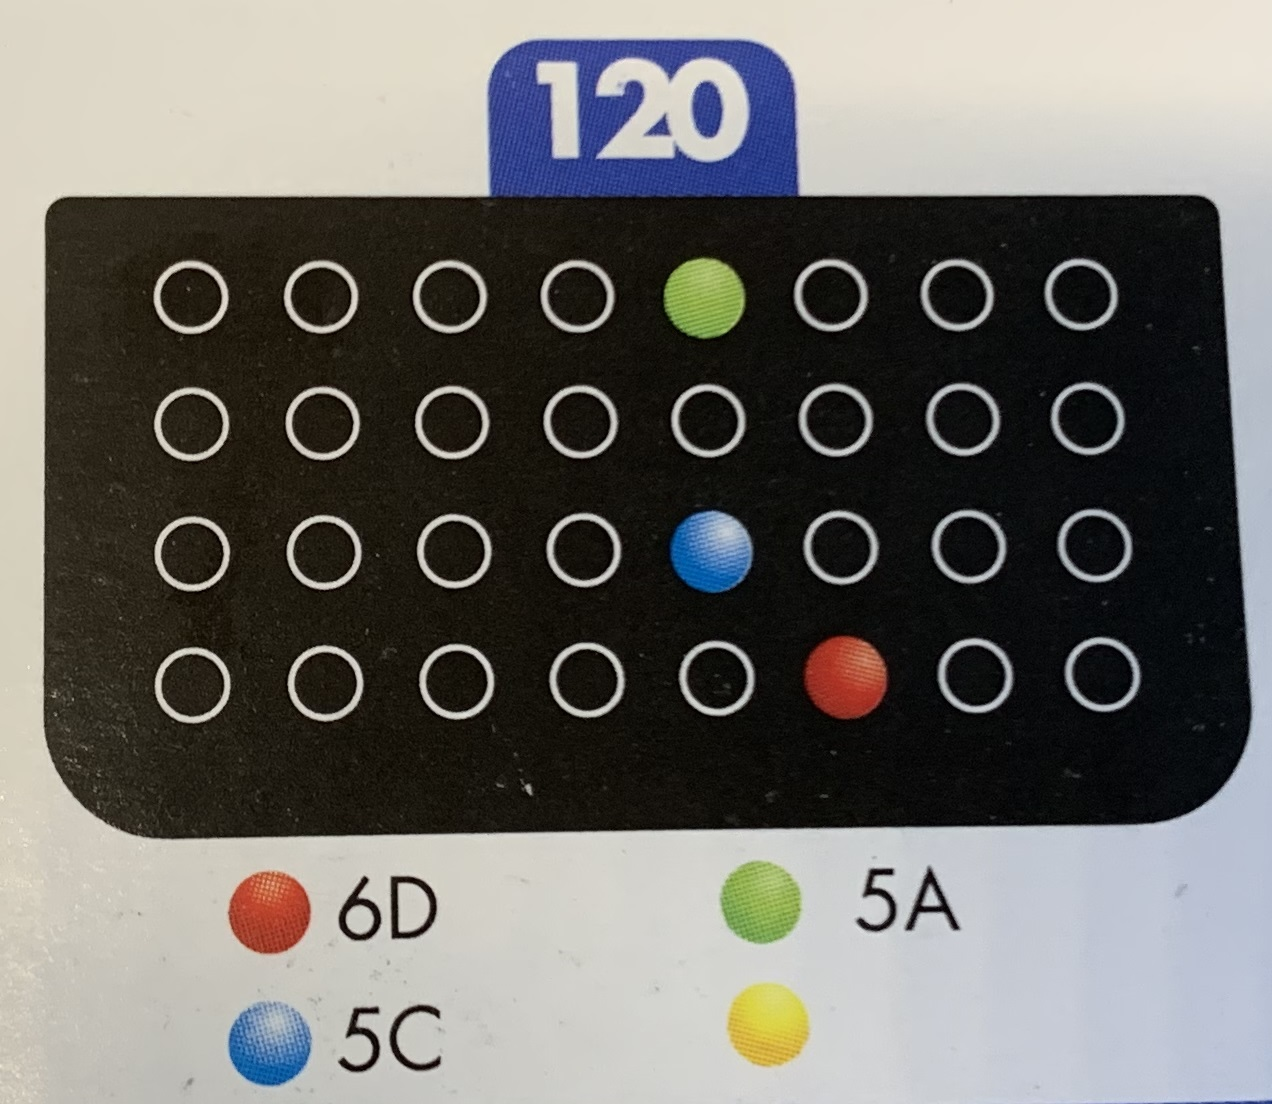
\includegraphics[width=0.6\textwidth]{figs/implementation1.jpg}
    \caption{The last problem in IQ Twist booklet}
    \label{fig:last_case}
\end{figure}
For example, with regard to the problem in Figure~\ref{fig:last_case}, it can be encoded by two parts, the position of the pegs, which is different for each problem, and the general CSP model introduced above, which is unique for all problems.
\subsubsection{Pegs' Position Information}
Figure~\ref{fig:last_case} shows there are only three pegs on the board. On account of the coordinate system in Figure~\ref{fig:coordinate}, the positions of blue peg, red peg, and green peg are separately placed on (5,2), (6,1) and (5,4). And the other pegs are not on the board. Hence, they could be encoded in Listing~\ref{lst:pegs' positions}.
\begin{lstlisting}[language=minizinc,numbers=none,caption={Encoding for pegs' positions},label={lst:pegs' positions}]
constraint Vpb1=52;
constraint Vpb2=0;  
constraint Vpg1=54;
constraint Vpg2=0;
constraint Vpy1=0;
constraint Vpy2=0;
constraint Vpr=61;
\end{lstlisting}
\bigskip
\smallbreak
\subsubsection{The General Model}
In this part, all the aspects such as variables, domains and constraints about the CSP model will be addressed.
\\Firstly, all variables in the CSP model are represented in Listing~\ref{lst:IQ Twist variables}.
\begin{lstlisting}[caption={Encoding for variables},label={lst:IQ Twist variables},language=minizinc,numbers=none]
var int:Vpr; var int:Vpb1;var int:Vpb2;var int:Vpg1;var int:Vpg2; var int:Vpy1;var int:Vpy2;
var position: Vb11;var position: Vb12;var position: Vb13;var position: Vb14;var position: Vb15;
var position: Vb21;var position: Vb22;var position: Vb23;var position: Vb24;
var position: Vg11;var position: Vg12;var position: Vg13;var position: Vg14;
var position: Vg21;var position: Vg22;var position: Vg23;
var position: Vr11;var position: Vr12;var position: Vr13;var position: Vr14; 
var position: Vr21;var position: Vr22;var position: Vr23;var position: Vr24;
var position: Vy11;var position: Vy12;var position: Vy13;
var position: Vy21;var position: Vy22;var position: Vy23;var position: Vy24;var position: Vy25;
\end{lstlisting}
\bigskip
\smallbreak
Secondly, the domain of $\VUnits$ is defined by "position" that corresponds to Listing~\ref{lst:IQ Twist domain}. In such a case, 11 in "position" means the position (1,1), 21 means the position (2,1) and so on.
\begin{lstlisting}[language=minizinc,numbers=none,caption={Encoding for pieces' domain},label={lst:IQ Twist domain}]
set of int: position={
14,24,34,44,54,64,74,84,
13,23,33,43,53,63,73,83,
12,22,32,42,52,62,72,82,
11,21,31,41,51,61,71,81};
\end{lstlisting}
\bigskip
\smallbreak
Furthermore, the constraints will be separately addressed. The code in Listing~\ref{lst:IQ Twist constraint1} represents the constraint in Equation~\ref{equ:firstconstrain}, which means there are no two different units of piece in the same position.
\begin{lstlisting}[language=minizinc,numbers=none,caption={Encoding for constraint one},label={lst:IQ Twist constraint1}]
constraint alldifferent([Vy11,Vy12,Vy13,Vy21,Vy22,Vy23,Vy24,Vy25,Vb11,Vb12,Vb13,Vb14,Vb15,Vb21,Vb22,Vb23,Vb24,Vg11,Vg12,Vg13,Vg14,
Vg21,Vg22,Vg23,Vr11,Vr12,Vr13,Vr14,Vr21,Vr22,Vr23,Vr24]);
\end{lstlisting}
\bigskip
\smallbreak
With regards to the second constraint in Equation~\ref{equ:secondconstrain}, because the positions for pegs have been set, the constraint is useless now.
\\For the third constraint in Equation~\ref{equ:thirdconstrain}, as an example for yellow2, it is encoded in Listing~\ref{lst:IQ Twist constraint3}.
\begin{lstlisting}[language=minizinc,numbers=none,caption={Encoding for constraint three},label={lst:IQ Twist constraint3}]
constraint (g0(Vy22) = g0(Vy21) + 1/\ g1(Vy22) = g1(Vy21)/\ g0(Vy23) = g0(Vy21) + 1/\ g1(Vy23) = g1(Vy21) + 1
            /\ g0(Vy24) = g0(Vy21) + 2/\ g1(Vy24) = g1(Vy21) + 1/\ g0(Vy25) = g0(Vy21) + 1/\ g1(Vy25) = g1(Vy21) + 2) \/
            
           (g0(Vy22) = g0(Vy21)/\ g1(Vy22) = g1(Vy21) + 1/\ g0(Vy23) = g0(Vy21) - 1/\ g1(Vy23) = g1(Vy21) + 1
            /\ g0(Vy24) = g0(Vy21) - 1/\ g1(Vy24) = g1(Vy21) + 2/\ g0(Vy25) = g0(Vy21) - 2/\ g1(Vy25) = g1(Vy21) + 1) \/
            
           (g0(Vy22) = g0(Vy21) - 1/\ g1(Vy22) = g1(Vy21)/\ g0(Vy23) = g0(Vy21) - 1/\ g1(Vy23) = g1(Vy21) - 1
            /\ g0(Vy24) = g0(Vy21) - 2/\ g1(Vy24) = g1(Vy21) - 1/\ g0(Vy25) = g0(Vy21) - 1/\ g1(Vy25) = g1(Vy21) - 2) \/
            
           (g0(Vy22) = g0(Vy21)/\ g1(Vy22) = g1(Vy21) - 1/\ g0(Vy23) = g0(Vy21) + 1/\ g1(Vy23) = g1(Vy21) - 1
            /\ g0(Vy24) = g0(Vy21) + 1/\ g1(Vy24) = g1(Vy21) - 2/\ g0(Vy25) = g0(Vy21) + 2/\ g1(Vy25) = g1(Vy21) - 1) \/
            
           (g0(Vy22) = g0(Vy21) - 1/\ g1(Vy22) = g1(Vy21)/\ g0(Vy23) = g0(Vy21) - 1/\ g1(Vy23) = g1(Vy21) + 1
            /\ g0(Vy24) = g0(Vy21) - 2/\ g1(Vy24) = g1(Vy21) + 1/\ g0(Vy25) = g0(Vy21) - 1/\ g1(Vy25) = g1(Vy21) + 2) \/
            
           (g0(Vy22) = g0(Vy21)/\ g1(Vy22) = g1(Vy21) - 1/\ g0(Vy23) = g0(Vy21) - 1/\ g1(Vy23) = g1(Vy21) - 1
            /\ g0(Vy24) = g0(Vy21) - 1/\ g1(Vy24) = g1(Vy21) - 2/\ g0(Vy25) = g0(Vy21) - 2/\ g1(Vy25) = g1(Vy21) - 1) \/
            
           (g0(Vy22) = g0(Vy21) + 1/\ g1(Vy22) = g1(Vy21)/\ g0(Vy23) = g0(Vy21) + 1/\ g1(Vy23) = g1(Vy21) - 1
            /\ g0(Vy24) = g0(Vy21) + 2/\ g1(Vy24) = g1(Vy21) - 1/\ g0(Vy25) = g0(Vy21) + 1/\ g1(Vy25) = g1(Vy21) - 2) \/
            
           (g0(Vy22) = g0(Vy21)/\ g1(Vy22) = g1(Vy21) + 1/\ g0(Vy23) = g0(Vy21) + 1/\ g1(Vy23) = g1(Vy21) + 1
            /\ g0(Vy24) = g0(Vy21) + 1/\ g1(Vy24) = g1(Vy21) + 2/\ g0(Vy25) = g0(Vy21) + 2/\ g1(Vy25) = g1(Vy21) + 1);
\end{lstlisting}
\bigskip
\smallbreak
In this constraint, because the positions are encoded as integers such as $(1,1)$ to 11, the g0 function is used to get the corresponding $y$ value and g1 function is used to get the corresponding $x$ value. Accordingly, the functions are represented in Listing~\ref{lst:IQ Twist functions}.
\begin{lstlisting}[language=minizinc,numbers=none,caption={Encoding for functions},label={lst:IQ Twist functions}]
function var int:g0(var int:a)=a mod 10;
function var int:g1(var int:a)=a div 10;
\end{lstlisting}
\bigskip
\smallbreak
Comparably, the other pieces can be encoded. For the last constraint in Equation~\ref{equ:fourthconstrain}, as an instance, the yellow peg1 can be encoded as below.
\begin{lstlisting}[language=minizinc,numbers=none,caption={Encoding for constraint four},label={lst:IQ Twist constraint4}]
constraint (Vpy1=00)\/(Vy11=Vpy1)\/(Vy21=Vpy1)\/(Vy22=Vpy1)\/(Vy24=Vpy1);
\end{lstlisting}
\bigskip
\smallbreak
In addition, other pegs can be represented in the same way.
\\By this way, the complete codes for the problem for Figure~\ref{fig:last_case} in Appendix~\ref{appendix:finalcaseIQtwist}. Similarly, all the other problems can be encoded in this way.
\section{Zig Zag Puzzler}
Zig Zag Puzzler is a 3D puzzle game with two playing modes. It consists of nine pieces. Figure~\ref{fig:ZIG_ZAG_Puzzler_playing_modes} shows that there are two boards, which correspond to different playing modes. Both modes use the same pieces and they aim to place all pieces to fully fill the game board. In addition, there are some pieces placed in advance to set the difficulty in each mode. The colored parts in Figure~\ref{fig:ZIG_ZAG_Puzzler_playing_modes} are the pieces that are placed in advance. Generally, the fewer pieces are placed in advance, the more difficult to solve the puzzle.
\begin{figure}[htbp]
    \centering
    \begin{subfigure}[b]{0.32\textwidth}
    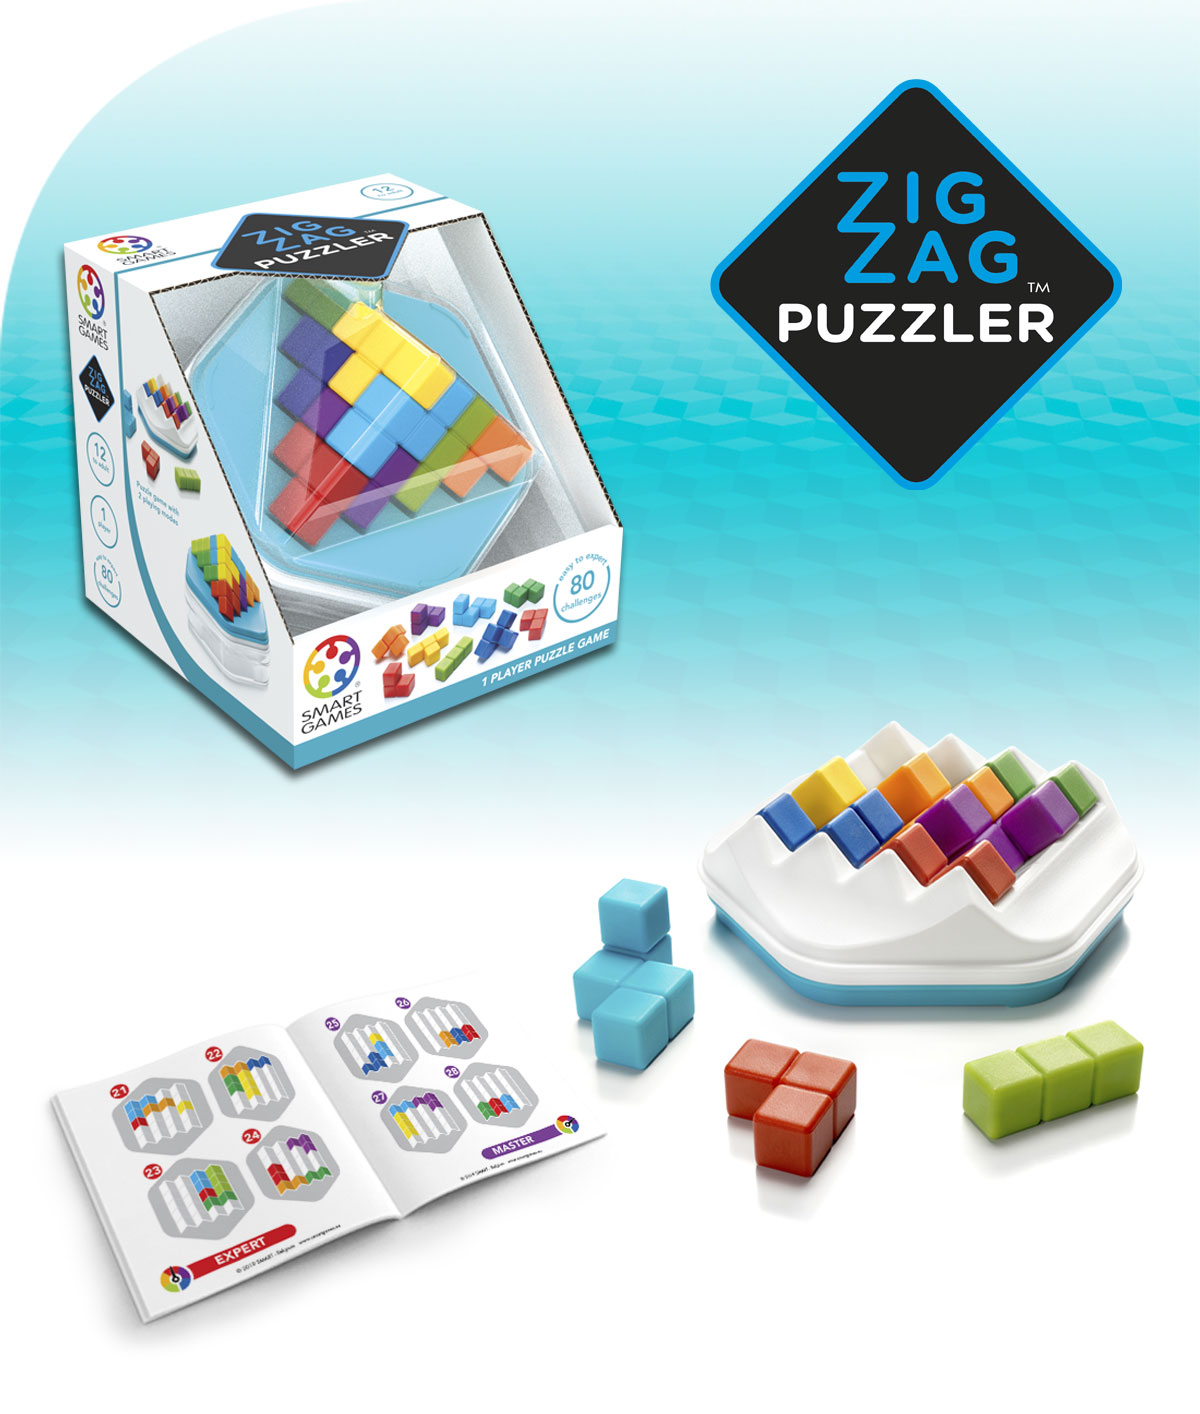
\includegraphics[width=\textwidth]{figs/zigzagdescription.jpg}
    \caption{Zig Zag Puzzler game}
    \end{subfigure}
    \begin{subfigure}[b]{0.32\textwidth}
    
\includegraphics[width=\textwidth]{figs/zig_zag_mode1.jpg}
    \caption{One example of playing mode 1}
    \end{subfigure}
    \begin{subfigure}[b]{0.32\textwidth}
    
\includegraphics[width=\textwidth]{figs/zig_zag_mode2.jpg}
    \caption{One example of playing mode 2}
    \end{subfigure}
    \caption{Zig Zag Puzzler examples, adopted from~\cite{r23}}
    \label{fig:ZIG_ZAG_Puzzler_playing_modes}
\end{figure}
In this part, the design of CSP models for Zig Zag Puzzler will be discussed. The two playing modes use the same pieces but different boards. Therefore, both playing modes will be based on the same coordinate system so that they can adopt the same variables and the same constraints but different domains. 
\subsection{Variables}
\begin{figure}[htbp]
\centering
\begin{subfigure}[b]{0.25\textwidth}
\centering
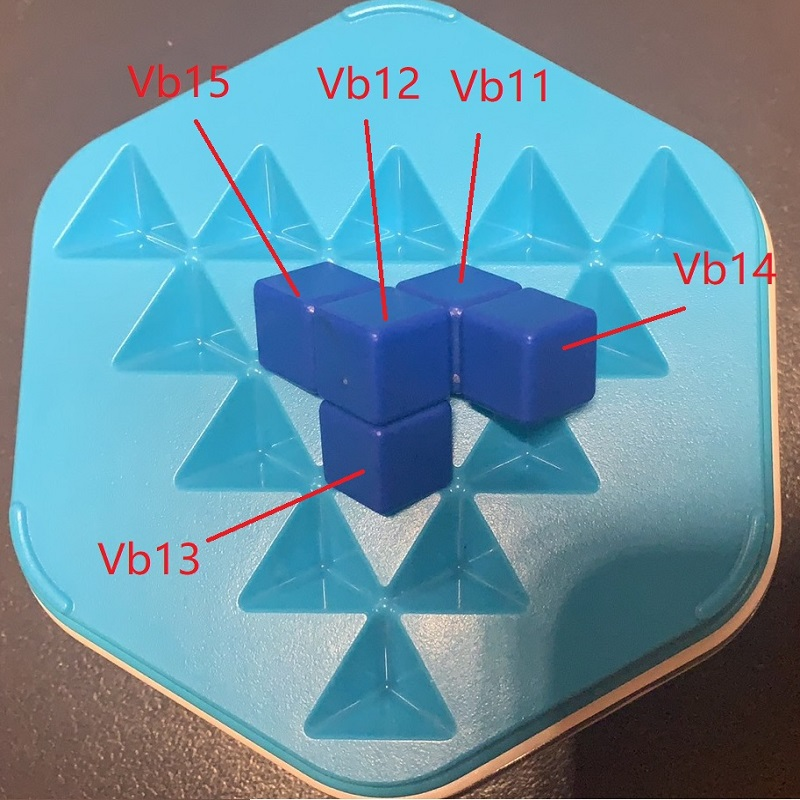
\includegraphics[width=\textwidth]{figs/3Dblue1.jpg}
\caption{Piece of variable $V_{b1}$}
  \label{fig:3Dblue1}
\end{subfigure}
\begin{subfigure}[b]{0.25\textwidth}
\centering
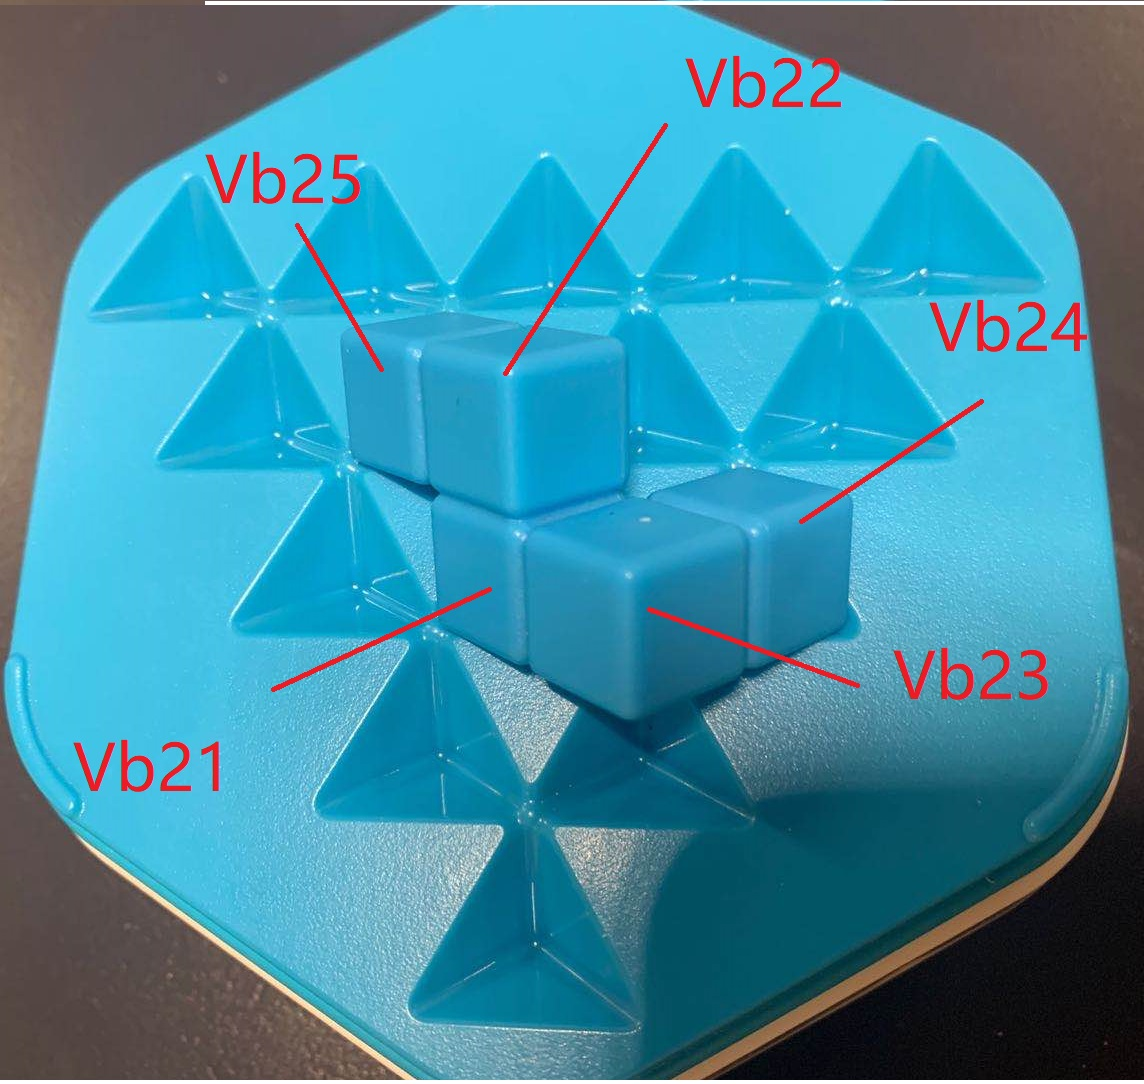
\includegraphics[width=\textwidth]{figs/3Dblue2.jpg}
\caption{Piece of variable $V_{b2}$}
  \label{fig:3Dblue2}
\end{subfigure}
\begin{subfigure}[b]{0.25\textwidth}
\centering
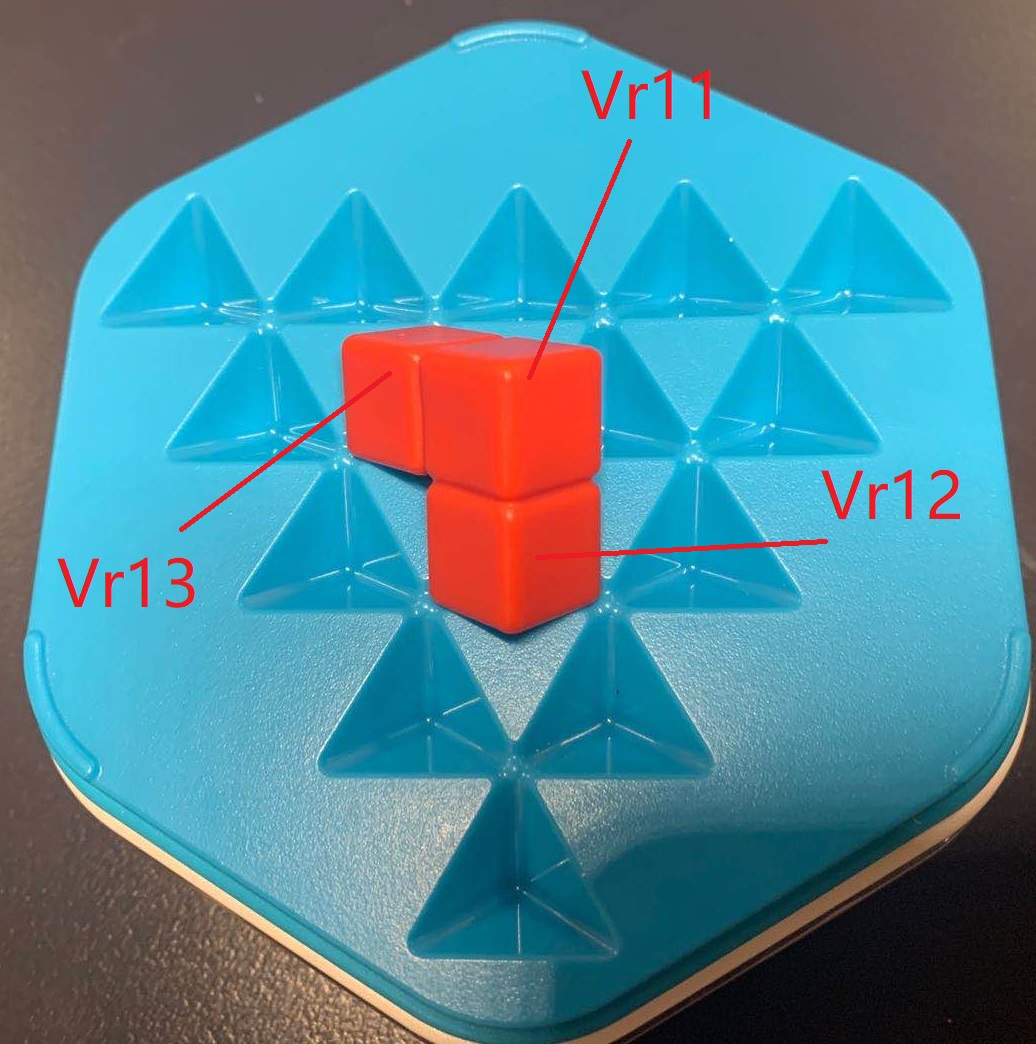
\includegraphics[width=\textwidth]{figs/3Dred1.jpg}
\caption{Piece of variable $V_{r1}$}
  \label{fig:3Dred1}
\end{subfigure}
\begin{subfigure}[b]{0.25\textwidth}
\centering
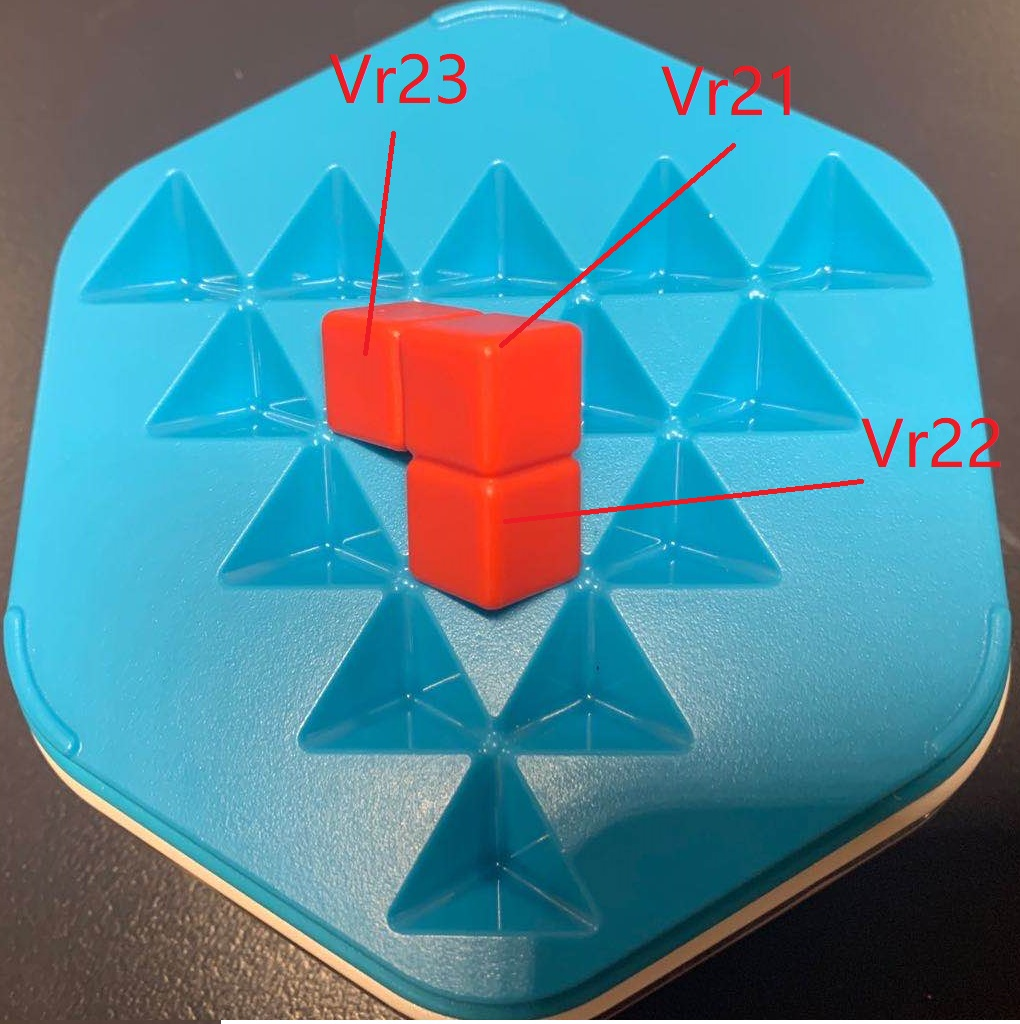
\includegraphics[width=\textwidth]{figs/3Dred2.jpg}
\caption{Piece of variable $V_{r2}$}
  \label{fig:3Dred2}
\end{subfigure}
\begin{subfigure}[b]{0.25\textwidth}
\centering
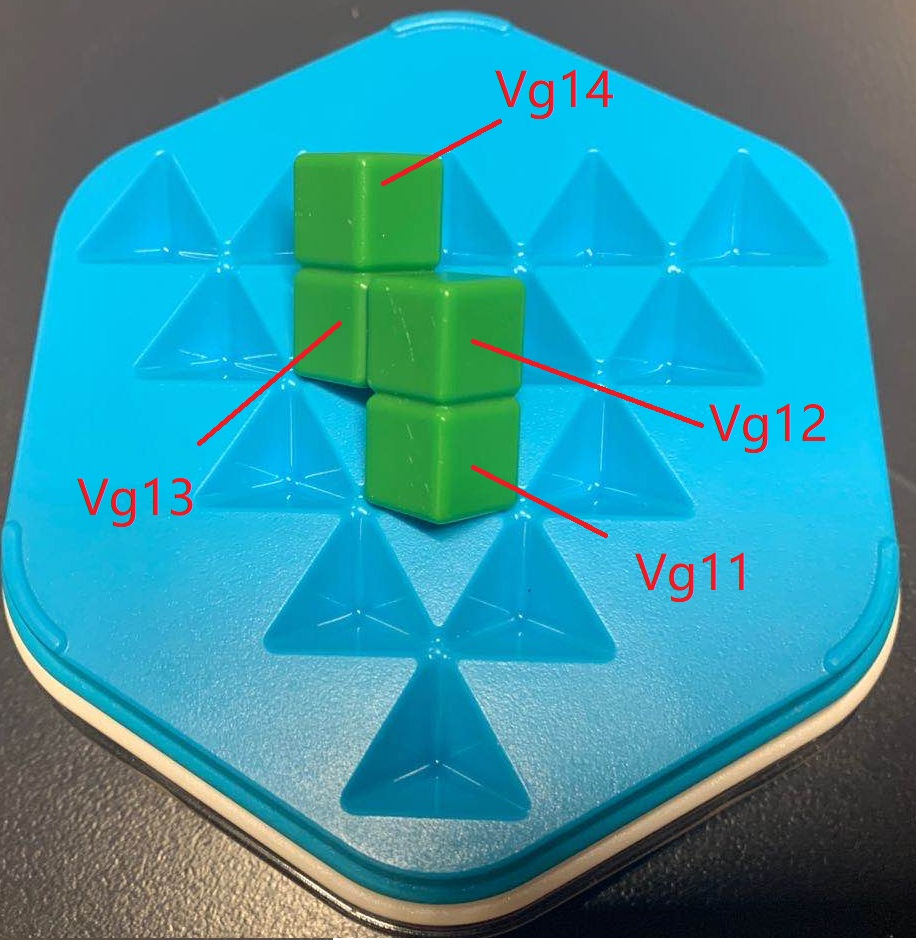
\includegraphics[width=\textwidth]{figs/3Dgreen1.jpg}
\caption{Piece of variable $V_{g1}$}
  \label{fig:3Dgreen1}
\end{subfigure}
\begin{subfigure}[b]{0.25\textwidth}
\centering
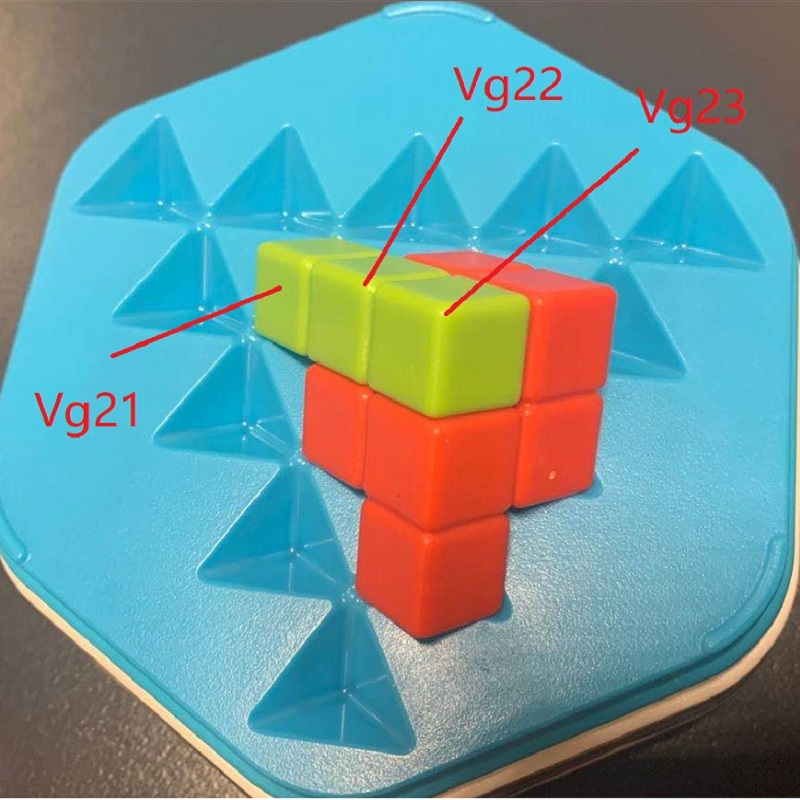
\includegraphics[width=\textwidth]{figs/3Dgreen2.jpg}
\caption{Piece of variable $V_{g2}$}
  \label{fig:3Dgreen2}
\end{subfigure}
\begin{subfigure}[b]{0.25\textwidth}
\centering
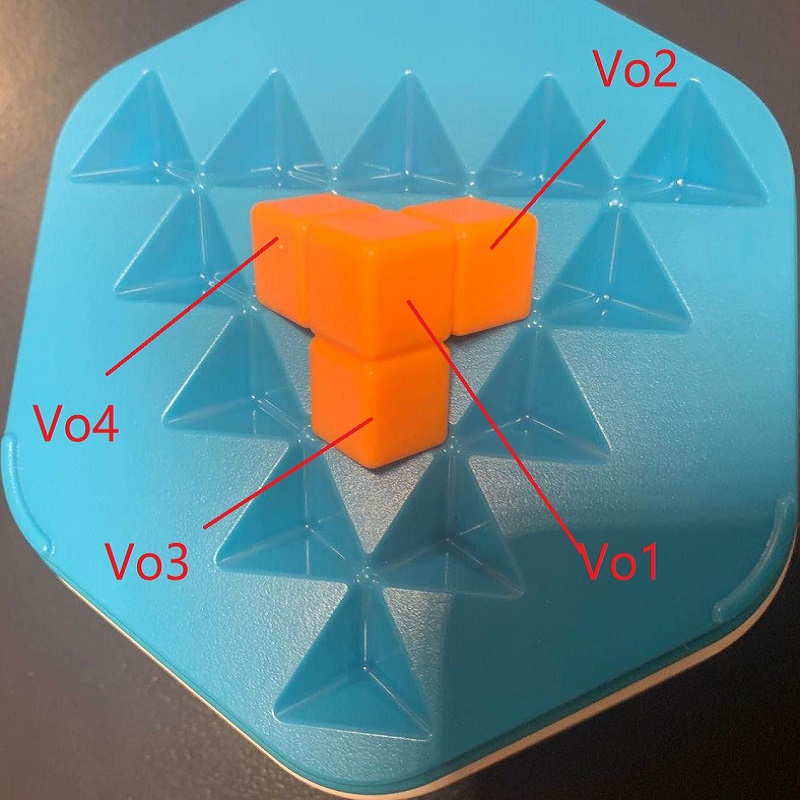
\includegraphics[width=\textwidth]{figs/3Dorange.jpg}
\caption{Piece of variable $V_{o}$}
  \label{fig:3Dorange}
\end{subfigure}
\begin{subfigure}[b]{0.25\textwidth}
\centering
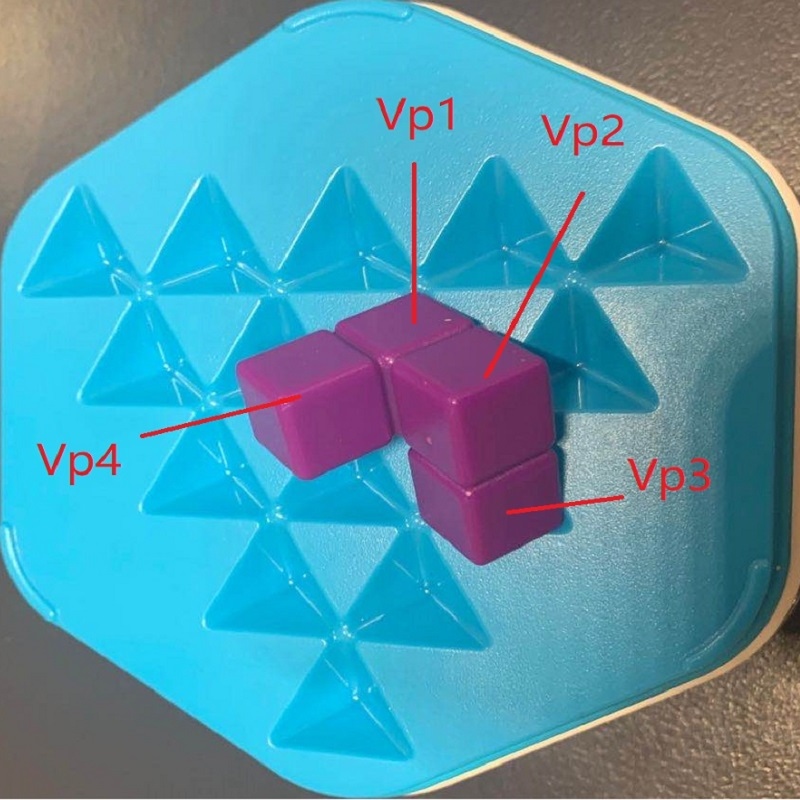
\includegraphics[width=\textwidth]{figs/3Dpurple.jpg}
\caption{Piece of variable $V_{p}$}
  \label{fig:3Dpurple}
\end{subfigure}
\begin{subfigure}[b]{0.25\textwidth}
\centering
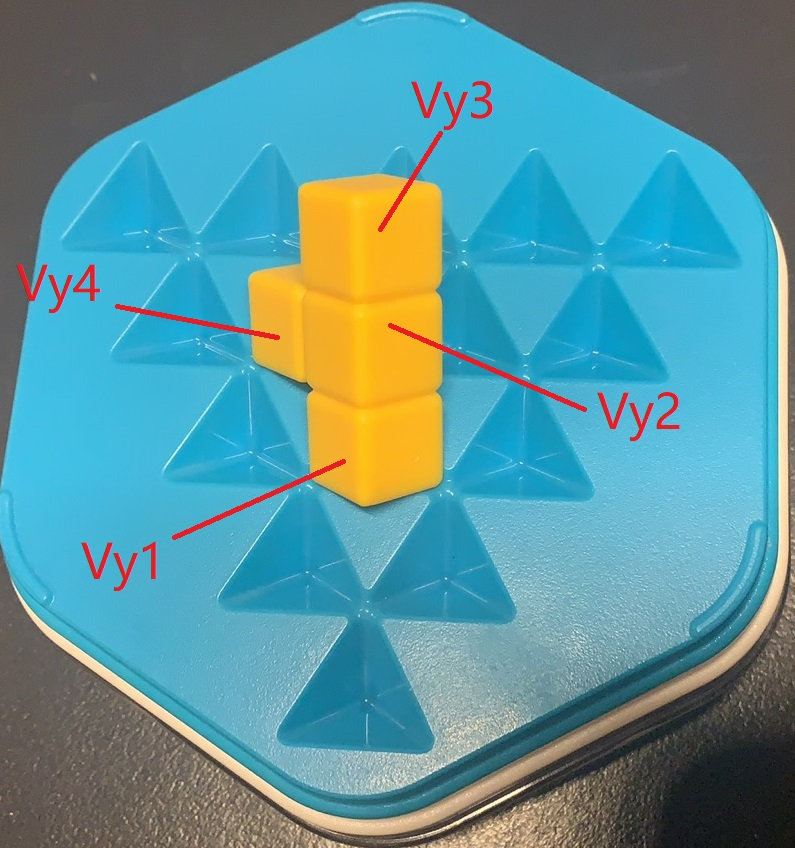
\includegraphics[width=\textwidth]{figs/3Dyellow.jpg}
\caption{Piece of variable $V_{y}$}
  \label{fig:3Dyellow}
\end{subfigure}
\caption{Initial state of each piece}
  \label{fig:all3Dinit}
\end{figure}
Firstly, the initial state of each piece is defined in Figure~\ref{fig:all3Dinit}.
It shows all the variables that are corresponding to the specific units. Therefore, the variables can be defined as
\begin{equation}
\begin{aligned}
\VUnits=\{&V_{y1},V_{y2},V_{y3},V_{y4},\\&V_{b11},V_{b12},V_{b13},V_{b14},
V_{b15},\\&V_{b21},V_{b22},V_{b23},V_{b24},V_{b25},\\&V_{g11},V_{g12},V_{g13},V_{g14},\\&V_{g21},V_{g22},V_{g23},\\&V_{r11},
V_{r12},V_{r13},\\&V_{r21},V_{r22},V_{r23},\\&V_{o1},V_{o2},V_{o3},V_{o4},\\&V_{p1},V_{p2},V_{p3},V_{p4}\}.
\end{aligned}
\end{equation}
\subsection{Domains for Playing Mode 1 and 2}
\label{sec:3Ddomains}
Figure~\ref{fig:board1} and Figure~\ref{fig:board2} show how to create the coordinate systems for both modes to represent the positions on the boards. In each Figure, there are two different visual angles to see the coordinate systems, which aims to explain the coordinate system more clearly. For both of them, similar to IQ Twist, the positions are represented as tuples and each tuple consists of three elements which are integers. The position of origin of coordinate can be represented as $(1,1,1)$. Now, one position on the board is considered as $(x_{0},y_{0},z_{0})$.
\begin{figure}[htbp]
\centering
\begin{subfigure}[b]{.45\textwidth}
\centering
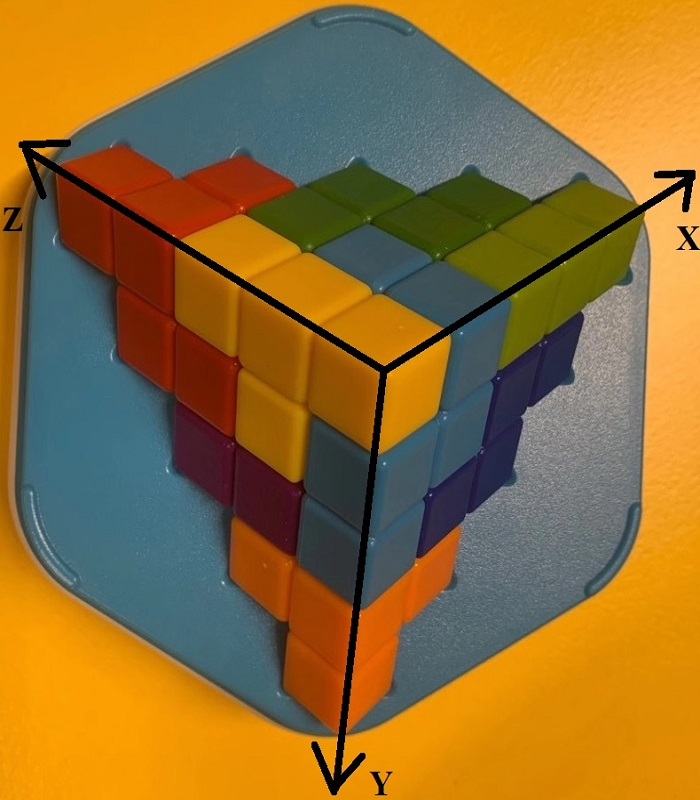
\includegraphics[width=\textwidth]{figs/ZIGZAGmodel1board.jpg}
\caption{}
\label{figure:mode1A}
\end{subfigure}
\begin{subfigure}[b]{.45\textwidth}
\centering
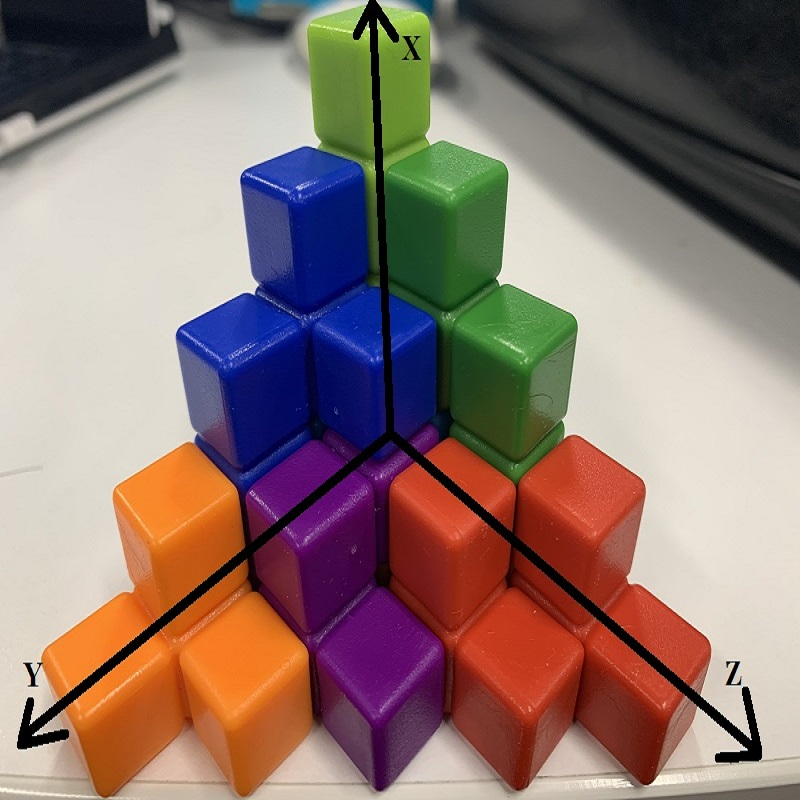
\includegraphics[width=\textwidth]{figs/3Dboard1.jpg}
\caption{}
\label{figure:mode1B}
\end{subfigure}
\caption{The board of Zig Zag Puzzler mode1}
  \label{fig:board1}
\end{figure}
\\For playing mode 1, as is shown in Figure~\ref{fig:board1}, the maximum number for each axis is 5, hence,
\begin{equation}
\begin{aligned}
&0<x_{0}\leq5,\\
&0<y_{0}\leq5,\\
&0<z_{0}\leq5.
\end{aligned}
\end{equation}
According to the structure of the cube in Figure~\ref{fig:board1}, if $(x_{0},y_{0},z_{0})$ is located in one of the three planes such as xy-plane which corresponds to the position $(x_{0},y_{0},1)$, it will satisfy
\begin{equation}
x_{0}+y_{0}\leq6.
\end{equation}
Accordingly, it will satisfy 
\begin{equation}
x_{0}+z_{0}\leq6
\end{equation}
in xz-plane and 
\begin{equation}
y_{0}+z_{0}\leq6
\end{equation}
in yz-plane. In addition, Figure~\ref{figure:mode1B} shows that although some units that are not on the 3 planes, there is only one unit distance to one of the three planes for each of them. So we get
\begin{equation}
x_{0}+y_{0}+z_{0}\leq7.
\end{equation}
Because what we discussed above has included all possible positions, the domain of playing mode 1 is
\begin{equation}
\begin{aligned}
&\forall \hspace{1ex} v \in \VUnits,\\
&D(v)=\{(x,y,z) \in \mathbb{N} \times \mathbb{N}	\times \mathbb{N} \mid  0<x \leq 5, \hspace{1ex} 0<y \leq 5,\hspace{1ex} 0<z \leq 5,\\ &x+y\leq 6,\hspace{1ex} y+z\leq 6,\hspace{1ex}x+z\leq 6,\hspace{1ex}x+y+z\leq 7\}.
\end{aligned}
\end{equation}
\begin{figure}[htbp]
\centering
\begin{subfigure}[b]{.45\textwidth}
\centering
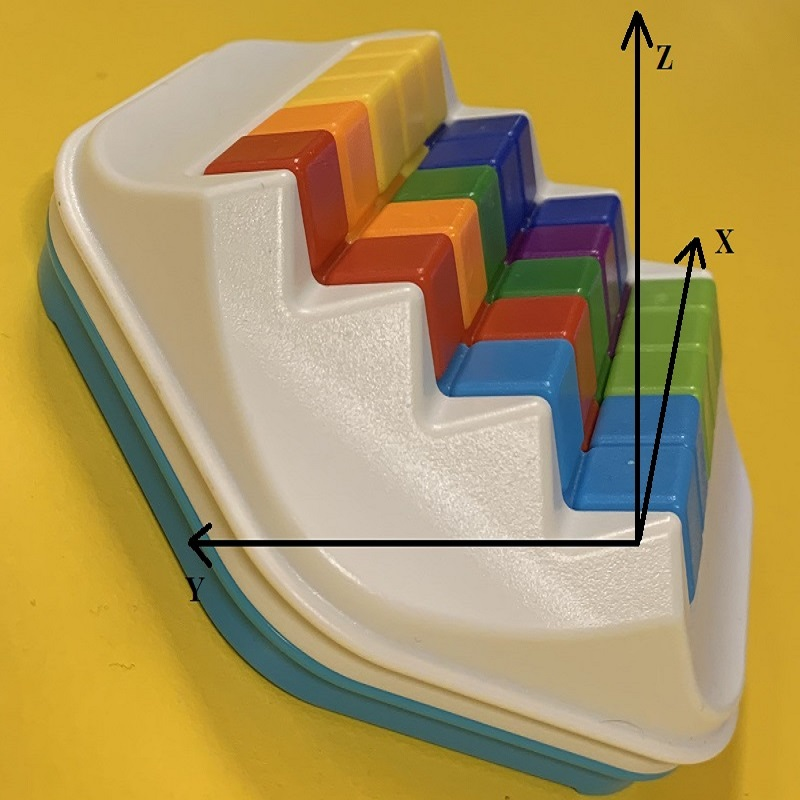
\includegraphics[width=\textwidth]{figs/ZIGZAGmodel2board.jpg}
\caption{}
\label{fig:board2A}
\end{subfigure}
\begin{subfigure}[b]{.45\textwidth}
\centering
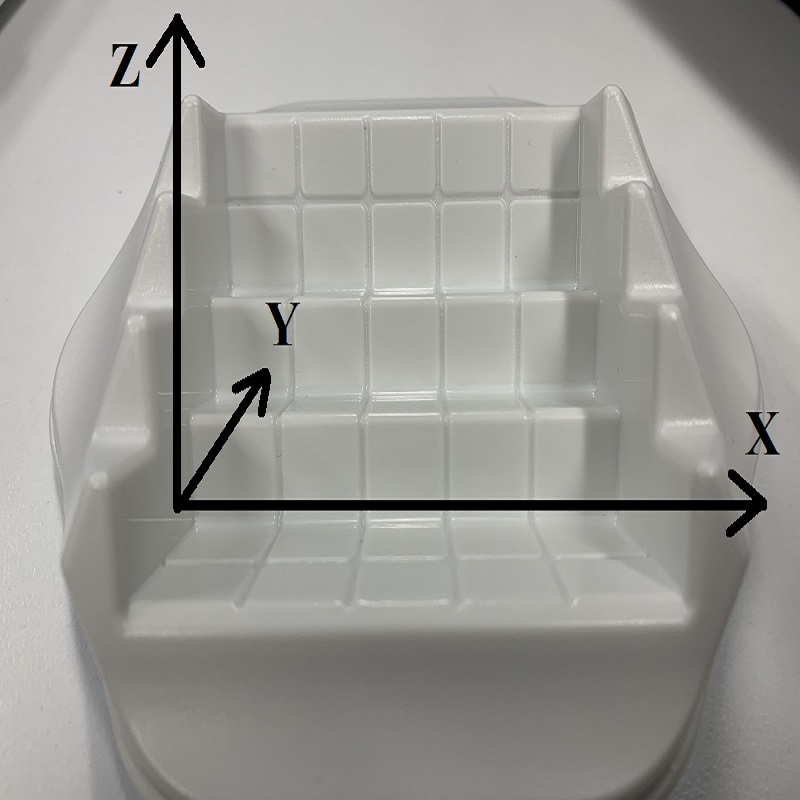
\includegraphics[width=\textwidth]{figs/3Dboard2.jpg}
\caption{}
\label{fig:board2B}
\end{subfigure}
\caption{The board of Zig Zag Puzzler mode2}
  \label{fig:board2}
\end{figure}
For playing mode 2, Figure~\ref{fig:board2} shows that the maximum number for both y-axis and z-axis are 4 and x-axis is 5, hence, 
\begin{equation}
\begin{aligned}
&0<x_{0}\leq5,\\
&0<y_{0}\leq4,\\
&0<z_{0}\leq4.
\end{aligned}
\end{equation}
In addition, the board is similar to stairs, if $(x_{0},y_{0},z_{0})$ is located in these positions, we can get
\begin{equation}
y_{0}=z_{0}.
\end{equation}
Besides the positions that is similar to stairs, the left space satisfy 
\begin{equation}
y_{0}=z_{0}+1,
\end{equation}
except when $z_{0}=4$.
Therefore, the domain of playing mode 2 is
\begin{equation}
\begin{aligned}
&\forall v \in \VUnits,\\
&D(v)=\{(x,y,z) \in \mathbb{N} \times \mathbb{N}	\times \mathbb{N} \mid  0<x \leq 5 , \hspace{1ex} 0<y \leq 4,\hspace{1ex} 0<z \leq 4,y=z\} \hspace{1ex}\cup\\
&\{(x,y,z) \in \mathbb{N} \times \mathbb{N}	\times \mathbb{N} \mid  0<x \leq 5, \hspace{1ex} 0<y \leq 4,\hspace{1ex} 0<z \leq 3,y=z+1\}.
\end{aligned}
\end{equation}
\subsection{3D Rotation Matrix}
\label{section:3Drotationmatrix}
To clarify how to obtain all configurations for each piece, the 3D rotation matrix will be introduced.
\begin{figure}[htbp]
\label{figure:3Dblue1}
\centering
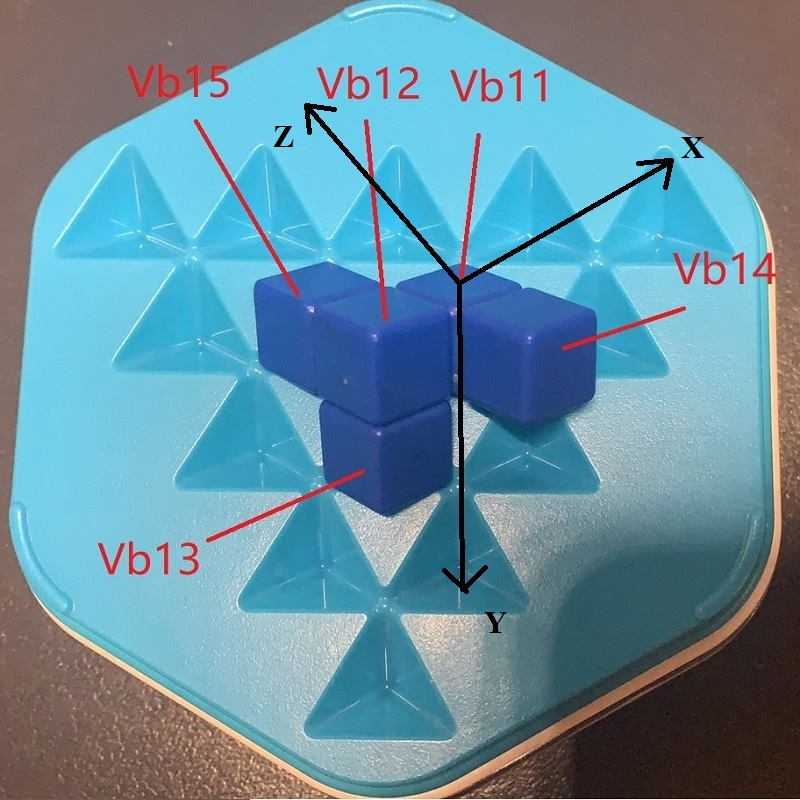
\includegraphics[width=0.3\textwidth]{figs/3Drotateexplain.jpg}
\caption{3Dblue1 initial state}
\label{fig:3Dblue1explanation}
\end{figure}
\\As is shown in Figure~\ref{fig:3Dblue1explanation}, the unit which is corresponding to the first variable $V_{b11}$ can be considered as a point $(x_{0},y_{0},z_{0})$. Considering a general case where a coordinate system includes negative values, if we assign $(0,0,0)$ to $(x_{0},y_{0},z_{0})$, on account of the coordinate system in Figure~\ref{fig:board1}, the $V_{b11}$, $V_{b12}$, $V_{b13}$, $V_{b14}$ and $V_{b15}$ are respectively represented as $(0,0,0)$, $(-1,0,0)$, $(-1,1,0)$, $(0,0,-1)$ and $(-1,0,1)$, which indicate that all other variables are connected with the first variables. For example, there are relationships
\begin{equation}
\begin{aligned}
&x_{V_{b11}}-1=x_{V_{b12}},\\
&y_{V_{b11}}=y_{V_{b12}},\\
&z_{V_{b11}}=z_{V_{b12}},
\end{aligned}
\end{equation}
between $V_{b11}$ and $V_{b12}$.
Similar to IQ Twist, the basic idea to find all configurations for each piece in Zig Zag Puzzler is all other units of the piece rotate around the first unit of the piece.
\\Tobias and Krantz \cite{r9} indicate that 3D rotations can be separately represented by rotation around x-axis, y-axis, and z-axis 
\begin{equation}
\label{equation:3Dmatrix1}
\begin{aligned}
R_{x}(\theta_{1})=\begin{bmatrix}
1&          0&          0\\
0&\cos\theta_{1} & -\sin\theta_{1}\\
0&\sin\theta_{1} & \cos\theta_{1}\\
\end{bmatrix},
\\R_{y}(\theta_{2})=\begin{bmatrix}
  \cos\theta_{2}&          0&\sin\theta_{2}\\
           0&          1& 0\\
-\sin\theta_{2} &          0&\cos\theta_{2}\\
\end{bmatrix},
\\R_{z}(\theta_{3})=\begin{bmatrix}
\cos\theta_{3}&-\sin\theta_{3}&0\\
\sin\theta_{3}& \cos\theta_{3}&0\\
         0&          0&1\\
\end{bmatrix},
\end{aligned}
\end{equation}
where $R_{x}(\theta_{1})$ is corresponding to counterclockwise rotation around x-axis by $\theta_{1}$, $R_{y}(\theta_{2})$ is corresponding to the counterclockwise rotation around y-axis by $\theta_{2}$ and $R_{z}(\theta_{3})$ is corresponding to the counterclockwise rotation around z-axis by $\theta_{3}$. In addition, if a point rotates around x-axis by $\alpha$, y-axis by $\beta$ and z-axis by $\gamma$ at the same time, the combination of the three matrices in Equation~\ref{equation:3Dmatrix1} can be represented as
\begin{equation}
\label{equation:3Dmatrix2}
\begin{aligned}
&R=R_{z}(\alpha)R_{y}(\beta)R_{x}(\gamma)=\\
&\begin{bmatrix}
\cos\alpha\cos\beta&\cos\alpha\sin\beta\sin\gamma-\sin\alpha\cos\gamma&\cos\alpha\sin\beta\cos\gamma+\sin\alpha\sin\gamma\\
\sin\alpha\cos\beta&\sin\alpha\sin\beta\sin\gamma+\cos\alpha\cos\gamma&\sin\alpha\sin\beta\cos\gamma-\cos\alpha\sin\gamma\\
         -\sin\beta&                               \cos\beta\sin\gamma&\cos\beta\cos\gamma\\
\end{bmatrix}.
\end{aligned}
\end{equation}
In our case, we only consider 0, 90, 180 and 270 degrees rotations for each axis. If we separately consider each axis, there should be four configurations for each. As an example, according to $R_{x}(\theta_{1})$ in Equation~\ref{equation:3Dmatrix1}, when the point(x,y,z) rotate around x-axis by $\theta_{1}$, we get
\begin{equation}
\begin{bmatrix}
x'\\
y'\\
z'\\
\end{bmatrix}
=R_{x}(\theta_{1})
\begin{bmatrix}
x\\
y\\
z\\
\end{bmatrix}
\end{equation}, which implies
\begin{equation}
\label{equation:theta1}
\begin{aligned}
&x'=x,\\
&y'=y\cos\theta_{1}-z\sin\theta_{1},\\
&z'=y\sin\theta_{1}+z\cos\theta_{1}.
\end{aligned}
\end{equation}
Therefore, if $0^{\circ}, 90^{\circ}, 180^{\circ}, 270^{\circ}$ are assigned to $\theta_{1}$ in Equation~\ref{equation:theta1}, we obtain $(x,y,z)$, $(x,-z,y)$, $(x,-y,-z)$ and $(x,z,-y)$.
Similarly, if a point rotates around the y-axis and the z-axis by $0^{\circ}$, $90^{\circ}$, $180^{\circ}$ and $270^{\circ}$, we can get four configurations each. Intuitively, the number of all possible configurations should be 64 because a point can rotate around x-axis by $\theta_{1}$ which is $0^{\circ}$, $90^{\circ}$, $180^{\circ}$ or $270^{\circ}$, rotate around y-axis by $\theta_{2}$ which is $0^{\circ}$, $90^{\circ}$, $180^{\circ}$ or $270^{\circ}$, and rotate around z-axis by $\theta_{3}$ which is $0^{\circ}$, $90^{\circ}$, $180^{\circ}$ or $270^{\circ}$. Therefore, all possible configurations should be the combination of $\theta_{1}$, $\theta_{2}$ and $\theta_{3}$, there should be a total of $4\times 4 \times 4$ configurations. 
\\However, there are only 24 configurations because of the "singularities" of Euler angles set. "A problem arises when using three-angle sequences and particular values of the middle angle leads to a condition called a singularity"~\cite{r29}. Euler angles are three angles that are used to represent the direction of rigid body in 3D space~\cite{r24}, which corresponds to $\alpha$, $\beta$ and $\gamma$ in Equation~\ref{equation:3Dmatrix2}. Hughes~\cite{r19} highlights that "any set of Euler angles where the second rotation aligns the axes of the first and third rotations causes a singularity". The second rotation axis is y-axis, and the corresponding rotation angles are $\beta$. In addition, the geometric singularities only appear when
$\beta=0^{\circ}$ and $180^{\circ}$ which is called "a repeated axis sequence" because the first and third axes are the same, and $\beta=\pm90^{\circ}$ which is called "non-repeated axis sequences"~\cite{r17,r19}. How do they cause singularities? 
\\Firstly, let us consider $\beta=\pm90^{\circ}$. If $\beta=90^{\circ}$, we get 
\begin{equation}
R_{\beta=90}=R_{z}(\alpha)R_{y}(90^{\circ})R_{x}(\gamma)=
\begin{bmatrix}
0&-\sin(\alpha-\gamma)&\cos(\alpha-\gamma)\\
0&\cos(\alpha-\gamma)&\sin(\alpha-\gamma)\\
         -1&                              0&0\\
\end{bmatrix}.
\end{equation}
And when $\beta=-90^{\circ}$, it can be seen as $\beta=270^{\circ}$ because of the periodicity, we can get 
\begin{equation}
R_{\beta=270}=R_{z}(\alpha)R_{y}(270^{\circ})R_{x}(\gamma)=
\begin{bmatrix}
0&-\sin(\alpha+\gamma)&-\cos(\alpha+\gamma)\\
0&\cos(\alpha+\gamma)&-\sin(\alpha+\gamma)\\
1&                               0&0
\end{bmatrix}.
\end{equation}
Based on the formula
\begin{equation}
\begin{bmatrix}
x'\\
y'\\
z'\\
\end{bmatrix}
=R
\begin{bmatrix}
x\\
y\\
z\\
\end{bmatrix},
\end{equation}
for $\beta=90^{\circ}$,
\begin{equation}
\label{equation:beta=90}
\begin{aligned}
&x'=-y\sin(\alpha-\gamma)-z\cos(\alpha-\gamma), \\
&y'=y\cos(\alpha-\gamma)+z\sin(\alpha-\gamma), \\
&z'=-x. 
\end{aligned}
\end{equation}
and for $\beta=270^{\circ}$, 
\begin{equation}
\label{equation:beta=270}
\begin{aligned}
&x'=-y\sin(\alpha+\gamma)-z\cos(\alpha+\gamma), \\
&y'=y\cos(\alpha+\gamma)-z\sin(\alpha+\gamma), \\
&z'=x.
\end{aligned}
\end{equation}
Because in our case, the possible values for both $\alpha$ and $\gamma$ are $0^{\circ}$, $90^{\circ}$, $180^{\circ}$ and $270^{\circ}$, and the period of the trigonometric function is $360^{\circ}$. For Equation~\ref{equation:beta=90}, the four situations are
\begin{equation}
\begin{aligned}
&\alpha-\gamma=0^{\circ},\\
&\alpha-\gamma=90^{\circ},\\
&\alpha-\gamma=180^{\circ},\\
&\alpha-\gamma=270^{\circ}.
\end{aligned}
\end{equation}
For Equation~\ref{equation:beta=270}, the four situations are 
\begin{equation}
\begin{aligned}
&\alpha+\gamma=0^{\circ},\\
&\alpha+\gamma=90^{\circ},\\
&\alpha+\gamma=180^{\circ},\\
&\alpha+\gamma=270^{\circ}.
\end{aligned}
\end{equation}
Therefore, these two groups of formulas represent that there are only four possible situations for each of them. What we should consider is $(\alpha-\gamma)$ in Equation~\ref{equation:beta=90} and $(\alpha+\gamma)$ in Equation~\ref{equation:beta=270}. 
\\In Equation~\ref{equation:beta=90}, we assign 0,90,180 and 270 degrees to the $(\alpha-\gamma)$, we get four configurations:
\begin{enumerate}
  \item  $x'=-y\sin(0^{\circ})-z\cos(0^{\circ}),\hspace{5pt} y'=y\cos(0^{\circ})+z\sin(0^{\circ}),\hspace{5pt} z'=-x \\\implies x'=-z,\hspace{5pt} y'=y,\hspace{5pt} z'=-x$
  \item  $x'=-y\sin(90^{\circ})-z\cos(90^{\circ}), \hspace{5pt} y'=y\cos(90^{\circ})+z\sin(90^{\circ}), \hspace{5pt} z'=-x\\\implies x'=-y,\hspace{5pt} y'=z,\hspace{5pt} z'=-x$
  \item  $x'=-y\sin(180^{\circ})-z\cos(180^{\circ}), \hspace{5pt} y'=y\cos(180^{\circ})+z\sin(180^{\circ}), \hspace{5pt} z'=-x\\\implies x'=z,\hspace{5pt} y'=-y,\hspace{5pt} z'=-x$
  \item  $x'=-y\sin(270^{\circ})-z\cos(270^{\circ}), \hspace{5pt} y'=y\cos(270^{\circ})+z\sin(270^{\circ}), \hspace{5pt} z'=-x\\\implies x'=y, \hspace{5pt}y'=-z,\hspace{5pt} z'=-x$
  \label{3Drotation24situations1}
\end{enumerate}
In Equation~\ref{equation:beta=270}, we assign 0,90,180 and 270 degrees to the $(\alpha+\gamma)$, we get four configurations:
\begin{enumerate}
\setcounter{enumi}{4}
  \item  $x'=-y\sin(0^{\circ})-z\cos(0^{\circ}),\hspace{5pt} y'=y\cos(0^{\circ})-z\sin(0^{\circ}),\hspace{5pt} z'=-x \\\implies x'=-z,\hspace{5pt} y'=y,\hspace{5pt} z'=x$
  \item  $x'=-y\sin(90^{\circ})-z\cos(90^{\circ}),\hspace{5pt} y'=y\cos(90^{\circ})-z\sin(90^{\circ}),\hspace{5pt} z'=-x\\\implies x'=-y,\hspace{5pt} y'=-z,\hspace{5pt} z'=x$
  \item  $x'=-y\sin(180^{\circ})-z\cos(180^{\circ}),\hspace{5pt} y'=y\cos(180^{\circ})-z\sin(180^{\circ}),\hspace{5pt} z'=-x\\\implies x'=z,\hspace{5pt} y'=-y,\hspace{5pt} z'=x$
  \item  $x'=-y\sin(270^{\circ})-z\cos(270^{\circ}),\hspace{5pt} y'=y\cos(270^{\circ})-z\sin(270^{\circ}),\hspace{5pt} z'=-x\\\implies x'=y, \hspace{5pt}y'=z,\hspace{5pt} z'=x$
  \label{3Drotation24situations2}
\end{enumerate}
Then, we consider  $\beta=0^{\circ}$ and $\beta=180^{\circ}$. Based on (3.6), when $\beta=0^{\circ}$, we get
\begin{equation}
\label{equation:beta=0}
R=R_{z}(\alpha)R_{y}(0^{\circ})R_{x}(\gamma)=
\begin{bmatrix}
\cos\alpha&-\sin\alpha\cos\gamma&\sin\alpha\sin\gamma\\
\sin\alpha&\cos\alpha\cos\gamma&-\cos\alpha\sin\gamma\\
0&          \sin\gamma&\cos\gamma\\
\end{bmatrix}.
\end{equation}
When $\beta=180^{\circ}$, we get
\begin{equation}
\label{equation:beta=180}
R=R_{z}(\alpha)R_{y}(180^{\circ})R_{x}(\gamma)=
\begin{bmatrix}
-\cos\alpha&-\sin\alpha\cos\gamma&\sin\alpha\sin\gamma\\
-\sin\alpha&\cos\alpha\cos\gamma&-\cos\alpha\sin\gamma\\
0&                               -\sin\gamma&-\cos\gamma\\
\end{bmatrix}.
\end{equation}
With regards to Equation~\ref{equation:beta=0} and Equation~\ref{equation:beta=180}, they are quite similar, the only difference is that Equation~\ref{equation:beta=180} contains more negative signs. Do they have any relationships? In Equation~\ref{equation:beta=180}, we assign $(\alpha+180^{\circ})$ to $\alpha$ and $(\gamma+180^{\circ})$ to $\gamma$, then it change to
\begin{equation}
\label{equation:alphaandgamma}
\begin{aligned}
&R=R_{z}(\alpha+180^{\circ})R_{y}(180^{\circ})R_{x}(\gamma+180^{\circ})=\\
&\begin{bmatrix}
-\cos(\alpha+180^{\circ})&-\sin(\alpha+180^{\circ})\cos(\gamma+180^{\circ})&\sin(\alpha+180^{\circ})\sin(\gamma+180^{\circ})\\
-\sin(\alpha+180^{\circ})&\cos(\alpha+180^{\circ})\cos(\gamma+180^{\circ})&-\cos(\alpha+180^{\circ})\sin(\gamma+180^{\circ})\\
0&                               -\sin(\gamma+180^{\circ})&-\cos(\gamma+180^{\circ})
\end{bmatrix}\\
&=\begin{bmatrix}
\cos(\alpha)&-\sin(\alpha)\cos(\gamma)&\sin(\alpha)\sin(\gamma)\\
\sin(\alpha)&\cos(\alpha)\cos(\gamma)&-\cos(\alpha)\sin(\gamma)\\
0&                               \sin(\gamma)&\cos(\gamma)\\
\end{bmatrix}.
\end{aligned}
\end{equation}
Therefore, based on Equation~\ref{equation:beta=0} and Equation~\ref{equation:alphaandgamma},
\begin{equation}
R_{z}(\alpha)R_{y}(0^{\circ})R_{x}(\gamma)=R_{z}(\alpha+180^{\circ})R_{y}(180^{\circ})R_{x}(\gamma+180^{\circ}),
\end{equation}
which means that for every configuration of $\alpha$ and $\gamma$ when $\beta=0^{\circ}$, there is an equivalent configuration at $\alpha+180$ and $\gamma+180$ when $\beta=180^{\circ}$. Even though the number of degrees of $\alpha+180^{\circ}$ or $\gamma+180^{\circ}$ may be more than $360^{\circ}$, it can always find a corresponding from $0^{\circ}$ to $360^{\circ}$ according to the periodicity of trigonometric function. For example, 
\begin{equation}
\begin{aligned}
&\circled{1}R_{z}(270^{\circ})Ry(0^{\circ})R_{x}(270^{\circ}) = R_{z}(450^{\circ})R_{y}(180^{\circ})R_{x}(450^{\circ}),\\ 
&\circled{2}R_{z}(450^{\circ})Ry(180^{\circ})R_{x}(450^{\circ}) = R_{z}(90^{\circ})R_{y}(180^{\circ})R_{x}(90^{\circ}),\\
&\circled{1},\circled{2}\implies R_{z}(270^{\circ})Ry(0^{\circ})R_{x}(270^{\circ})   = R_{z}(90^{\circ})R_{y}(180^{\circ})R_{x}(90^{\circ}).
\end{aligned}
\end{equation}
Hence, each combination among 
\begin{equation}
\begin{aligned}
&\beta=0^{\circ};\\
&\theta=0^{\circ}, 90^{\circ}, 180^{\circ}, 270^{\circ};\\
&\gamma=0^{\circ}, 90^{\circ}, 180^{\circ}, 270^{\circ};
\end{aligned}
\end{equation}
always corresponds to one combination among 
\begin{equation}
\begin{aligned}
&\beta=180^{\circ};\\
&\theta=0^{\circ}, 90^{\circ}, 180^{\circ}, 270^{\circ};\\
&\gamma=0^{\circ}, 90^{\circ}, 180^{\circ}, 270^{\circ}.
\end{aligned}
\end{equation}
So we only need to consider all configurations when $\beta=0^{\circ}$ because the all possible configurations in $\beta=180^{\circ}$ are duplicates. For Equation~\ref{equation:beta=0}, we assign $\theta=0^{\circ},\gamma=0^{\circ}$; $\theta=0^{\circ},\gamma=90^{\circ}$;...;$\theta=270^{\circ},\gamma=180^{\circ}$; $\theta=270^{\circ},\gamma=270^{\circ}$. we get
\begin{enumerate}
  \setcounter{enumi}{8}
  \item  $x'=x$,   $y'=y$,    $z'=z$,
  \item  $x'=x$,   $y'=-z$,   $z'=y$, 
  \item  $x'=x$,   $y'=-y$,   $z'=-z$, 
  \item  $x'=x$,   $y'=z$,    $z'=-y$,
  \item  $x'=-y$,  $y'=x$,    $z'=z$,
  \item  $x'=z$,   $y'=x$,    $z'=y$,
  \item  $x'=y$,   $y'=x$,    $z'=-z$,
  \item  $x'=-z$,  $y'=x$,    $z'=-y$,
  \item  $x'=-x$,  $y'=-y$,   $z'=z$,
  \item  $x'=-x$,  $y'=z$,    $z'=y$,
  \item  $x'=-x$,  $y'=y$,    $z'=-z$,
  \item  $x'=-x$,  $y'=-z$,   $z'=-y$,
  \item  $x'=y$,   $y'=-x$,   $z'=z$,
  \item  $x'=-z$,  $y'=-x$,   $z'=y$,
  \item  $x'=-y$,  $y'=-x$,   $z'=-z$,
  \item  $x'=z$,   $y'=-x$,   $z'=-y$.
  \label{3Drotation24situations3}
\end{enumerate}
There should be a total of 16 configurations (4$\times$4). Finally, consider the all configurations in $\beta=90^{\circ}$, $\beta=270^{\circ}$, $\beta=^{\circ}0$ and $\beta=180^{\circ}$. There should be a total of 4+4+16=24 configurations.
Therefore, if we assign $(0,0,0)$ to $Vb11$ in Figure~\ref{fig:3Dblue1explanation}, accordingly, we can get the initial states for $Vb12$, $Vb13$, $Vb14$ and $Vb15$. They separately correspond to (-1,0,0), (-1,-1,0), (0,0,-1) and (-1,0,1). 
All of them make up the initial state of Blue piece1. Based on the initial state of Blue piece1, if all other units of the piece rotate around $Vb11$, there should be 24 configurations. Considering the domains of Zig Zag Puzzler again, the piece can be moved as long as all units of piece on the board. Hence, on the condition of all units of piece on the board, we can assign variables $(x_{0},y_{0},z_{0})$ to $Vb11$, accordingly, we can get other units of piece's positions. Therefore, the constrains can be represented by the relationships between each other unit of piece with the first unit of piece $Vb11$. The specific constraint is shown below.
\subsection{Constraints}
Firstly, according to chapter~\ref{section:3Drotationmatrix}, there are 24 rotation configurations. So we get
\begin{align*}
&\Cons{b11}{b12}{b13}{b14}{b15}=\{((x_{1},y_{1},z_{1}),(x_{2},y_{2},z_{2}),(x_{3},y_{3},z_{3}),(x_{4},y_{4},z_{4}),(x_{5},y_{5},z_{5}))\in \\
&\Domain {b11} \times \Domain{b12}\times \Domain{b13}\times \Domain{b14}\times \Domain{b15} \mid\\
&(x_{2}=x_{1}-1,\hspace{1ex} y_{2}=y_{1},\hspace{1ex} z_{2}=z_{1},\hspace{1ex} x_{3}=x_{1}-1,\hspace{1ex} y_{3}=y_{1}+1,\hspace{1ex} z_{3}=z_{1},\hspace{1ex} x_{4}=x_{1},\\
&\hspace{1ex} y_{4}=y_{1},\hspace{1ex} z_{4}=z_{1}-1,\hspace{1ex} x_{5}=x_{1}-1,\hspace{1ex} y_{5}=y_{1},\hspace{1ex} z_{5}=z_{1}+1)&or\\ 
&(x_{2}=x_{1},\hspace{1ex} y_{2}=y_{1}+1,\hspace{1ex} z_{2}=z_{1},\hspace{1ex} x_{3}=x_{1},\hspace{1ex} y_{3}=y_{1}+1,\hspace{1ex} z_{3}=z_{1}-1,\hspace{1ex} x_{4}=x_{1}-1,\\
&\hspace{1ex} y_{4}=y_{1},\hspace{1ex} z_{4}=z_{1},\hspace{1ex} x_{5}=x_{1}+1,\hspace{1ex} y_{5}=y_{1}+1,\hspace{1ex} z_{5}=z_{1})&or\\ 
&(x_{2}=x_{1},\hspace{1ex} y_{2}=y_{1}+1,\hspace{1ex} z_{2}=z_{1},\hspace{1ex} x_{3}=x_{1},\hspace{1ex} y_{3}=y_{1}+1,\hspace{1ex} z_{3}=z_{1}+1,\hspace{1ex} x_{4}=x_{1}+1,\\
&\hspace{1ex} y_{4}=y_{1},\hspace{1ex} z_{4}=z_{1},\hspace{1ex} x_{5}=x_{1}-1,\hspace{1ex} y_{5}=y_{1}+1,\hspace{1ex} z_{5}=z_{1})&or\\ 
&(x_{2}=x_{1},\hspace{1ex} y_{2}=y_{1},\hspace{1ex} z_{2}=z_{1}-1,\hspace{1ex} x_{3}=x_{1}-1,\hspace{1ex} y_{3}=y_{1},\hspace{1ex} z_{3}=z_{1}-1,\hspace{1ex} x_{4}=x_{1},\\
&\hspace{1ex} y_{4}=y_{1}+1,\hspace{1ex} z_{4}=z_{1},\hspace{1ex} x_{5}=x_{1},\hspace{1ex} y_{5}=y_{1}-1,\hspace{1ex} z_{5}=z_{1}-1)&or\\ 
&(x_{2}=x_{1}-1,\hspace{1ex} y_{2}=y_{1},\hspace{1ex} z_{2}=z_{1},\hspace{1ex} x_{3}=x_{1}-1,\hspace{1ex} y_{3}=y_{1}-1,\hspace{1ex} z_{3}=z_{1},\hspace{1ex} x_{4}=x_{1},\\
&\hspace{1ex} y_{4}=y_{1},\hspace{1ex} z_{4}=z_{1}+1,\hspace{1ex} x_{5}=x_{1}-1,\hspace{1ex} y_{5}=y_{1},\hspace{1ex} z_{5}=z_{1}-1)&or\\ 
&(x_{2}=x_{1}+1,\hspace{1ex} y_{2}=y_{1},\hspace{1ex} z_{2}=z_{1},\hspace{1ex} x_{3}=x_{1}+1,\hspace{1ex} y_{3}=y_{1}-1,\hspace{1ex} z_{3}=z_{1},\hspace{1ex} x_{4}=x_{1},\\
&\hspace{1ex} y_{4}=y_{1},\hspace{1ex} z_{4}=z_{1}-1,\hspace{1ex} x_{5}=x_{1}+1,\hspace{1ex} y_{5}=y_{1},\hspace{1ex} z_{5}=z_{1}+1)&or\\ 
&(x_{2}=x_{1},\hspace{1ex} y_{2}=y_{1}-1,\hspace{1ex} z_{2}=z_{1},\hspace{1ex} x_{3}=x_{1},\hspace{1ex} y_{3}=y_{1}-1,\hspace{1ex} z_{3}=z_{1}-1,\hspace{1ex} x_{4}=x_{1}+1,\\
&\hspace{1ex} y_{4}=y_{1},\hspace{1ex} z_{4}=z_{1},\hspace{1ex} x_{5}=x_{1}-1,\hspace{1ex} y_{5}=y_{1}-1,\hspace{1ex} z_{5}=z_{1})&or\\ 
&(x_{2}=x_{1},\hspace{1ex} y_{2}=y_{1}-1,\hspace{1ex} z_{2}=z_{1},\hspace{1ex} x_{3}=x_{1},\hspace{1ex} y_{3}=y_{1}-1,\hspace{1ex} z_{3}=z_{1}+1,\hspace{1ex} x_{4}=x_{1}-1,\\
&\hspace{1ex} y_{4}=y_{1},\hspace{1ex} z_{4}=z_{1},\hspace{1ex} x_{5}=x_{1}+1,\hspace{1ex} y_{5}=y_{1}-1,\hspace{1ex} z_{5}=z_{1})&or\\ 
&(x_{2}=x_{1},\hspace{1ex} y_{2}=y_{1}+1,\hspace{1ex} z_{2}=z_{1},\hspace{1ex} x_{3}=x_{1}+1,\hspace{1ex} y_{3}=y_{1}+1,\hspace{1ex} z_{3}=z_{1},\hspace{1ex} x_{4}=x_{1},\\
&\hspace{1ex} y_{4}=y_{1},\hspace{1ex} z_{4}=z_{1}-1,\hspace{1ex} x_{5}=x_{1},\hspace{1ex} y_{5}=y_{1}+1,\hspace{1ex} z_{5}=z_{1}+1)&or\\ 
&(x_{2}=x_{1},\hspace{1ex} y_{2}=y_{1},\hspace{1ex} z_{2}=z_{1}+1,\hspace{1ex} x_{3}=x_{1},\hspace{1ex} y_{3}=y_{1}-1,\hspace{1ex} z_{3}=z_{1}+1,\hspace{1ex} x_{4}=x_{1}+1,\\
&\hspace{1ex} y_{4}=y_{1},\hspace{1ex} z_{4}=z_{1},\hspace{1ex} x_{5}=x_{1}-1,\hspace{1ex} y_{5}=y_{1},\hspace{1ex} z_{5}=z_{1}+1)&or\\ 
&(x_{2}=x_{1},\hspace{1ex} y_{2}=y_{1},\hspace{1ex} z_{2}=z_{1}+1,\hspace{1ex} x_{3}=x_{1}+1,\hspace{1ex} y_{3}=y_{1},\hspace{1ex} z_{3}=z_{1}+1,\hspace{1ex} x_{4}=x_{1},\\
&\hspace{1ex} y_{4}=y_{1}+1,\hspace{1ex} z_{4}=z_{1},\hspace{1ex} x_{5}=x_{1},\hspace{1ex} y_{5}=y_{1}-1,\hspace{1ex} z_{5}=z_{1}+1)&or\\ 
&(x_{2}=x_{1},\hspace{1ex} y_{2}=y_{1},\hspace{1ex} z_{2}=z_{1}-1,\hspace{1ex} x_{3}=x_{1},\hspace{1ex} y_{3}=y_{1}+1,\hspace{1ex} z_{3}=z_{1}-1,\hspace{1ex} x_{4}=x_{1}+1,\\
&\hspace{1ex} y_{4}=y_{1},\hspace{1ex} z_{4}=z_{1},\hspace{1ex} x_{5}=x_{1}-1,\hspace{1ex} y_{5}=y_{1},\hspace{1ex} z_{5}=z_{1}-1)&or\\ 
&(x_{2}=x_{1},\hspace{1ex} y_{2}=y_{1}-1,\hspace{1ex} z_{2}=z_{1},\hspace{1ex} x_{3}=x_{1}-1,\hspace{1ex} y_{3}=y_{1}-1,\hspace{1ex} z_{3}=z_{1},\hspace{1ex} x_{4}=x_{1},\\
&\hspace{1ex} y_{4}=y_{1},\hspace{1ex} z_{4}=z_{1}-1,\hspace{1ex} x_{5}=x_{1},\hspace{1ex} y_{5}=y_{1}-1,\hspace{1ex} z_{5}=z_{1}+1)&or\\ 
&(x_{2}=x_{1}+1,\hspace{1ex} y_{2}=y_{1},\hspace{1ex} z_{2}=z_{1},\hspace{1ex} x_{3}=x_{1}+1,\hspace{1ex} y_{3}=y_{1},\hspace{1ex} z_{3}=z_{1}-1,\hspace{1ex} x_{4}=x_{1},\\
&\hspace{1ex} y_{4}=y_{1}+1,\hspace{1ex} z_{4}=z_{1},\hspace{1ex} x_{5}=x_{1}+1,\hspace{1ex} y_{5}=y_{1}-1,\hspace{1ex} z_{5}=z_{1})&or\\
&(x_{2}=x_{1}+1,\hspace{1ex} y_{2}=y_{1},\hspace{1ex} z_{2}=z_{1},\hspace{1ex} x_{3}=x_{1}+1,\hspace{1ex} y_{3}=y_{1}+1,\hspace{1ex} z_{3}=z_{1},\hspace{1ex} x_{4}=x_{1},\\
&\hspace{1ex} y_{4}=y_{1},\hspace{1ex} z_{4}=z_{1}+1,\hspace{1ex} x_{5}=x_{1}+1,\hspace{1ex} y_{5}=y_{1},\hspace{1ex} z_{5}=z_{1}-1)&or\\ 
&(x_{2}=x_{1},\hspace{1ex} y_{2}=y_{1},\hspace{1ex} z_{2}=z_{1}-1,\hspace{1ex} x_{3}=x_{1},\hspace{1ex} y_{3}=y_{1}-1,\hspace{1ex} z_{3}=z_{1}-1,\hspace{1ex} x_{4}=x_{1}-1,\\
&\hspace{1ex} y_{4}=y_{1},\hspace{1ex} z_{4}=z_{1},\hspace{1ex} x_{5}=x_{1}+1,\hspace{1ex} y_{5}=y_{1},\hspace{1ex} z_{5}=z_{1}-1)&or\\ 
&(x_{2}=x_{1},\hspace{1ex} y_{2}=y_{1},\hspace{1ex} z_{2}=z_{1}+1,\hspace{1ex} x_{3}=x_{1},\hspace{1ex} y_{3}=y_{1}+1,\hspace{1ex} z_{3}=z_{1}+1,\hspace{1ex} x_{4}=x_{1}-1,\\
&\hspace{1ex} y_{4}=y_{1},\hspace{1ex} z_{4}=z_{1},\hspace{1ex} x_{5}=x_{1}+1,\hspace{1ex} y_{5}=y_{1},\hspace{1ex} z_{5}=z_{1}+1)&or\\ 
&(x_{2}=x_{1},\hspace{1ex} y_{2}=y_{1},\hspace{1ex} z_{2}=z_{1}-1,\hspace{1ex} x_{3}=x_{1}+1,\hspace{1ex} y_{3}=y_{1},\hspace{1ex} z_{3}=z_{1}-1,\hspace{1ex} x_{4}=x_{1},\\
&\hspace{1ex} y_{4}=y_{1}-1,\hspace{1ex} z_{4}=z_{1},\hspace{1ex} x_{5}=x_{1},\hspace{1ex} y_{5}=y_{1}+1,\hspace{1ex} z_{5}=z_{1}-1)&or\\ 
&(x_{2}=x_{1},\hspace{1ex} y_{2}=y_{1}-1,\hspace{1ex} z_{2}=z_{1},\hspace{1ex} x_{3}=x_{1}+1,\hspace{1ex} y_{3}=y_{1}-1,\hspace{1ex} z_{3}=z_{1},\hspace{1ex} x_{4}=x_{1},\\
&\hspace{1ex} y_{4}=y_{1},\hspace{1ex} z_{4}=z_{1}+1,\hspace{1ex} x_{5}=x_{1},\hspace{1ex} y_{5}=y_{1}-1,\hspace{1ex} z_{5}=z_{1}-1)&or\\ 
&(x_{2}=x_{1},\hspace{1ex} y_{2}=y_{1}+1,\hspace{1ex} z_{2}=z_{1},\hspace{1ex} x_{3}=x_{1}-1,\hspace{1ex} y_{3}=y_{1}+1,\hspace{1ex} z_{3}=z_{1},\hspace{1ex} x_{4}=x_{1},\\
&\hspace{1ex} y_{4}=y_{1},\hspace{1ex} z_{4}=z_{1}+1,\hspace{1ex} x_{5}=x_{1},\hspace{1ex} y_{5}=y_{1}+1,\hspace{1ex} z_{5}=z_{1}-1)&or\\ 
&(x_{2}=x_{1}+1,\hspace{1ex} y_{2}=y_{1},\hspace{1ex} z_{2}=z_{1},\hspace{1ex} x_{3}=x_{1}+1,\hspace{1ex} y_{3}=y_{1},\hspace{1ex} z_{3}=z_{1}+1,\hspace{1ex} x_{4}=x_{1},\\
&\hspace{1ex} y_{4}=y_{1}-1,\hspace{1ex} z_{4}=z_{1},\hspace{1ex} x_{5}=x_{1}+1,\hspace{1ex} y_{5}=y_{1}+1,\hspace{1ex} z_{5}=z_{1})&or\\ 
&(x_{2}=x_{1}-1,\hspace{1ex} y_{2}=y_{1},\hspace{1ex} z_{2}=z_{1},\hspace{1ex} x_{3}=x_{1}-1,\hspace{1ex} y_{3}=y_{1},\hspace{1ex} z_{3}=z_{1}+1,\hspace{1ex} x_{4}=x_{1},\\
&\hspace{1ex} y_{4}=y_{1}+1,\hspace{1ex} z_{4}=z_{1},\hspace{1ex} x_{5}=x_{1}-1,\hspace{1ex} y_{5}=y_{1}-1,\hspace{1ex} z_{5}=z_{1})&or\\ 
&(x_{2}=x_{1},\hspace{1ex} y_{2}=y_{1},\hspace{1ex} z_{2}=z_{1}+1,\hspace{1ex} x_{3}=x_{1}-1,\hspace{1ex} y_{3}=y_{1},\hspace{1ex} z_{3}=z_{1}+1,\hspace{1ex} x_{4}=x_{1},\\
&\hspace{1ex} y_{4}=y_{1}-1,\hspace{1ex} z_{4}=z_{1},\hspace{1ex} x_{5}=x_{1},\hspace{1ex} y_{5}=y_{1}+1,\hspace{1ex} z_{5}=z_{1}+1)&or\\ 
&(x_{2}=x_{1}-1,\hspace{1ex} y_{2}=y_{1},\hspace{1ex} z_{2}=z_{1},\hspace{1ex} x_{3}=x_{1}-1,\hspace{1ex} y_{3}=y_{1},\hspace{1ex} z_{3}=z_{1}-1,\hspace{1ex} x_{4}=x_{1},\\
&\hspace{1ex} y_{4}=y_{1}-1,\hspace{1ex} z_{4}=z_{1},\hspace{1ex} x_{5}=x_{1}-1,\hspace{1ex} y_{5}=y_{1}+1,\hspace{1ex} z_{5}=z_{1})\}.
\end{align*}
Similarly, we can get the constraints for other pieces.
\\Secondly, there should be no two different units of piece take up the same position
\begin{equation}
\label{equ:3Dfirstconstrain}
\begin{aligned}
&\forall v_{m},v_{n} \in \VUnits\quad \text{where} \quad v_{m} \neq v_{n}:\\
&\Constraints{m}{n}=\{((x_{1},y_{1},z_{1}),(x_{2},y_{2},z_{2}))\in \Domain{m} \times \Domain{n}\mid x_{1} \neq x_{2}   \hspace{1ex} or \hspace{1ex}  y_{1} \neq y_{2} \hspace{1ex} or \hspace{1ex}  z_{1} \neq z_{2}\}.
\end{aligned}
\end{equation}
\subsection{Encodings for Zig Zag Puzzler}
All problems in the Zig Zag Puzzler booklet are encoded in Minizinc. For both playing mode 1 and playing mode 2, some pieces will be set on the board in advance. Therefore, each problem can be considered as two parts, one is the placed pieces which is different for each problem, the other is the general CSP model which is unique for all problems. 
\subsubsection{Placed Pieces}
\begin{figure}[htbp]
    \centering
    \begin{subfigure}[b]{.45\textwidth}
    \centering
    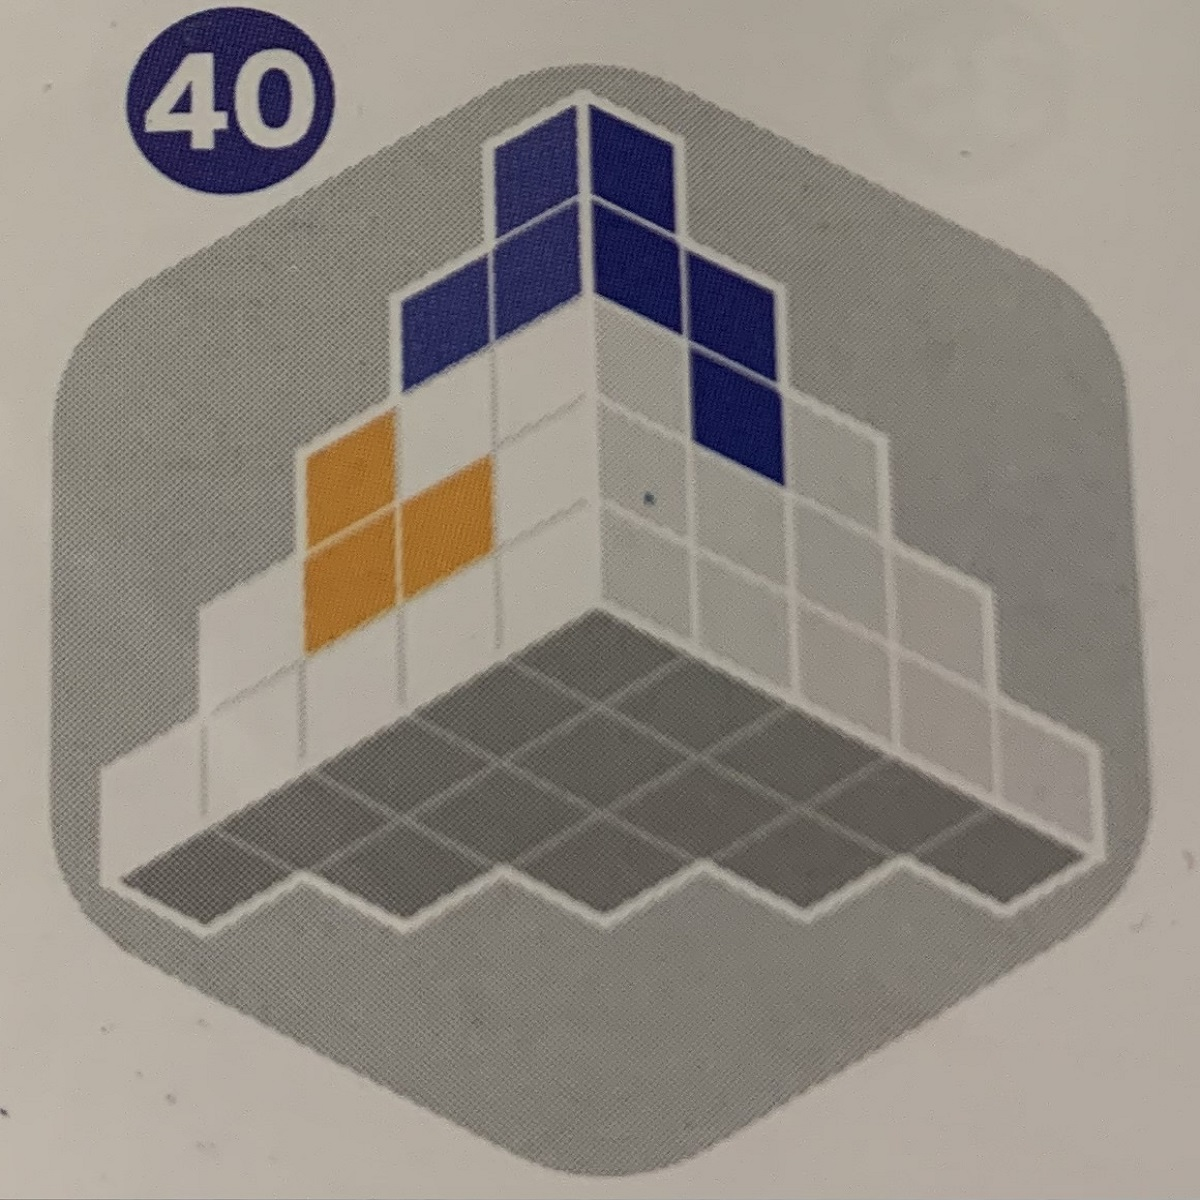
\includegraphics[width=\textwidth]{figs/mode1.jpg}
    \caption{The last problem in Zig Zag Puzzler playing mode 1}
    \label{fig:game2mode1}
    \end{subfigure}
     \begin{subfigure}[b]{.45\textwidth}
     \centering
      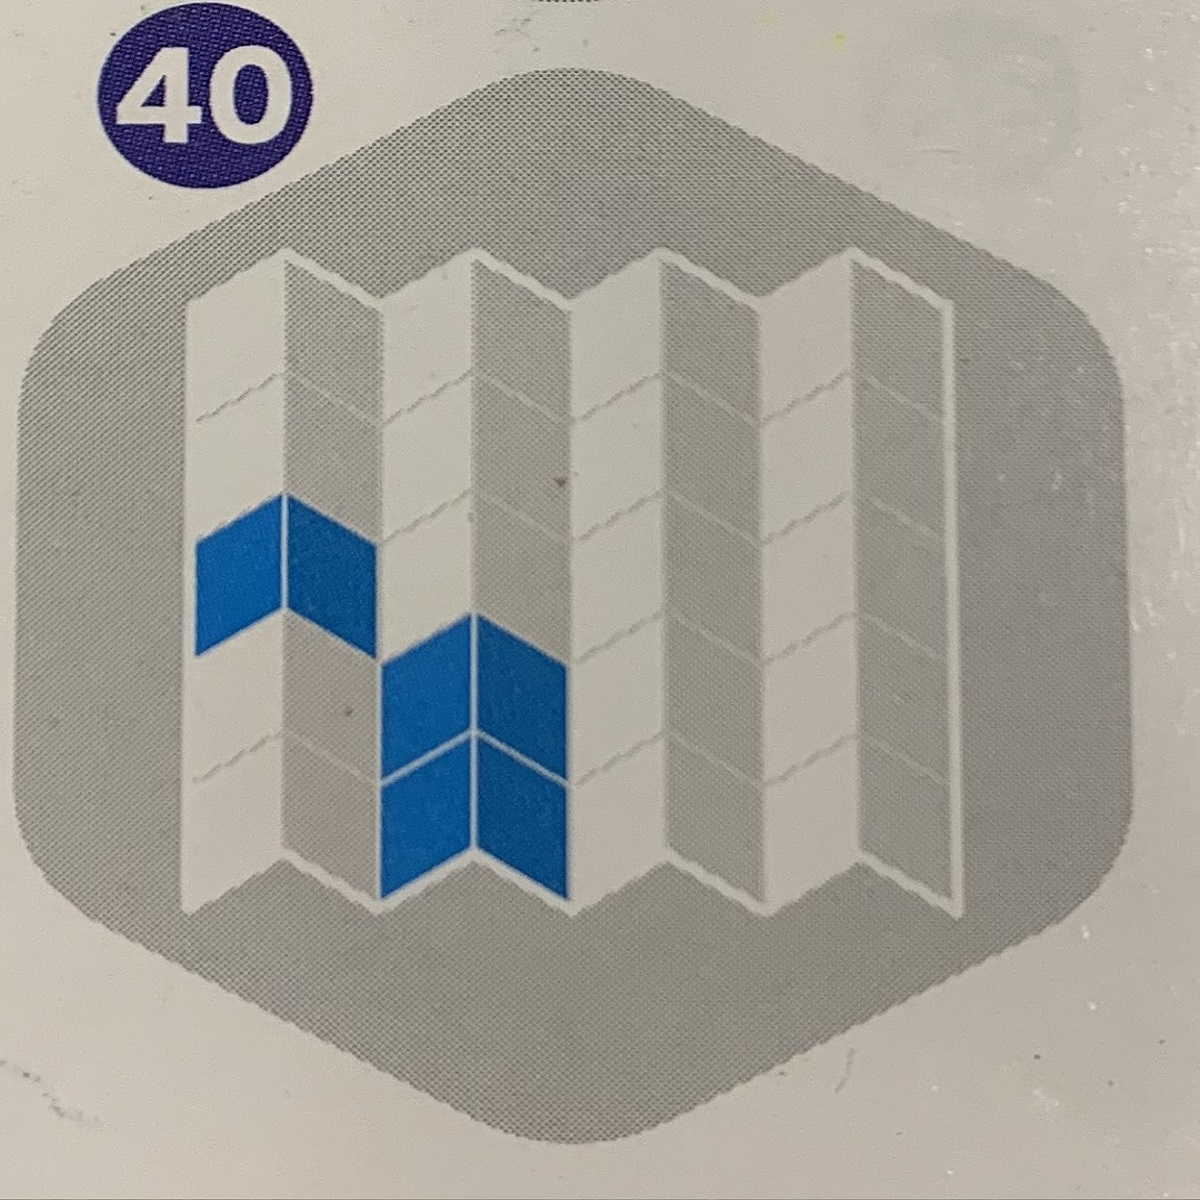
\includegraphics[width=\textwidth]{figs/mode2.jpg}
    \caption{The last problem in Zig Zag Puzzler playing mode 2}
    \label{fig:game2mode2}
     \end{subfigure}
     \caption{The examples in Zig Zag Puzzler}
     \label{fig:exampleszigzag}
\end{figure}
Figure~\ref{fig:game2mode1} shows the last problem in Zig Zag Puzzler playing mode 1. According to the board in Figure~\ref{fig:board1} and the pieces in Figure~\ref{fig:3Dblue1} and Figure~\ref{fig:3Dorange}, the positions of the units of blue piece1 $Vb11$, $Vb12$, $Vb13$, $Vb14$ and $Vb15$ are $(1,4,2)$, $(1,4,1)$, $(2,4,1)$, $(1,3,2)$ and $(1,5,1)$, which are encoded as Listing~\ref{lst:Bluepiece1}.
\begin{lstlisting}[language=minizinc,numbers=none,caption={Encoding for blue piece1's position of last problem in playing mode 1},label={lst:Bluepiece1}]
constraint Vb11 = 142;
constraint Vb12 = 141;
constraint Vb13 = 241;
constraint Vb14 = 132;
constraint Vb15 = 151;
\end{lstlisting}
\bigskip
\smallbreak
And the positions of the units of orange piece $Vo1$, $Vo2$, $Vo3$ and $Vo4$ are $(3,2,1)$, $(3,3,1)$, $(2,2,1)$ and $(3,2,2)$, which are encoded as Listing~\ref{lst:Orangepiece}.
\begin{lstlisting}[language=minizinc,numbers=none,caption={Encoding for orange piece's position of last problem in playing mode 1},label={lst:Orangepiece}]
constraint Vo1 = 321;
constraint Vo2 = 331;
constraint Vo3 = 221;
constraint Vo4 = 322;
\end{lstlisting}
\bigskip
\smallbreak
Figure~\ref{fig:game2mode2} shows the last problem in Zig Zag Puzzler playing mode 2. Based on the board in Figure~\ref{fig:board2} and the pieces in Figure~\ref{fig:3Dblue1}, the position of the units of blue piece Vb21, Vb22, Vb23, Vb24 and Vb25 are $(2,4,3)$, $(2,3,3)$, $(3,4,3)$, $(3,4,4)$ and $(1,3,3)$, which are encoded as Listing~\ref{lst:Blue2piece}.
\begin{lstlisting}[language=minizinc,numbers=none,caption={Encoding for blue piece2's position of last problem in playing mode 2},label={lst:Blue2piece}]
constraint Vb21 = 243;
constraint Vb22 = 233;
constraint Vb23 = 343;
constraint Vb24 = 344;
constraint Vb25 = 133;
\end{lstlisting}
\bigskip
\smallbreak
In addition, for the playing mode 2, there might be some special problems.
\begin{figure}[htbp]
    \centering
    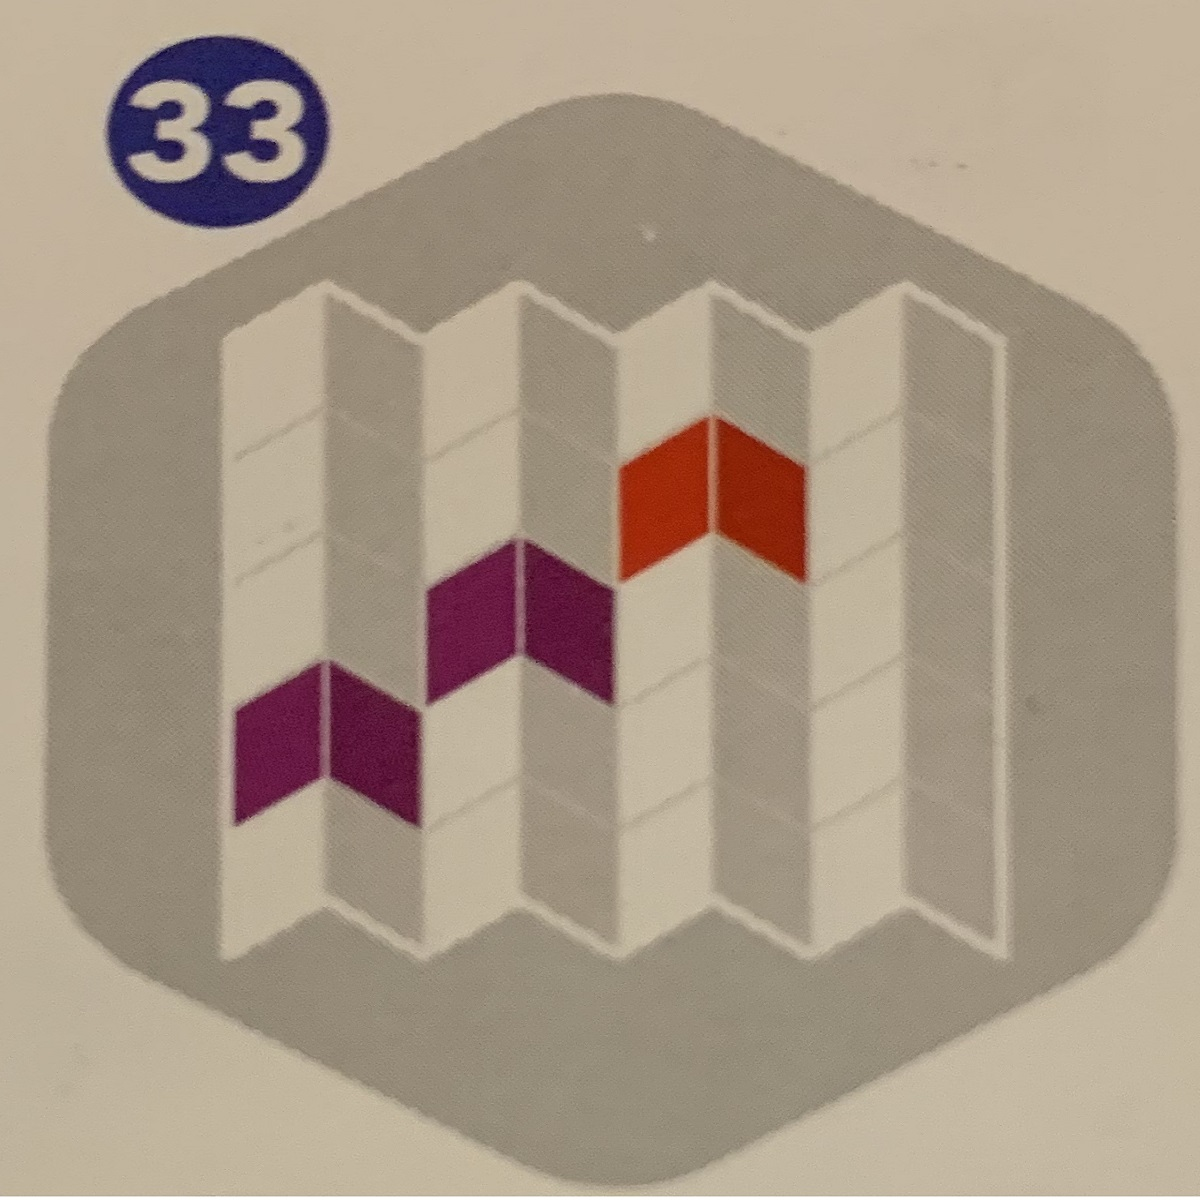
\includegraphics[width=0.4\textwidth]{figs/specialcase.jpg}
    \caption{The special problem in Zig Zag Puzzler playing mode 2}
    \label{fig:specialcase}
\end{figure}
For instance, in Figure~\ref{fig:specialcase}, it's hard to judge where are the exact positions of units of red piece. In such a case, the red piece1 (although red piece1 and red piece2 are exactly the same shape, we assume it is red piece1 here) can be encoded as Listing~\ref{lst:red1}.
\begin{lstlisting}[language=minizinc,numbers=none,caption={Encoding for red piece1's position of special problem},label={lst:red1}]
constraint (Vr11=422 \/  Vr12=422);
\end{lstlisting}
\bigskip
\smallbreak
It means that we only get the information $Vr11=422$ or $Vr12=422$ from Figure~\ref{fig:specialcase}, the other units of the piece's positions are unknown.
\subsubsection{The General Model}
In this part, all the aspects about CSP model will be addressed.
\\Firstly, for both playing modes, the variables are encoded as Listing~\ref{lst:variables}.
\begin{lstlisting}[language=minizinc,numbers=none,caption={Encoding for variables},label={lst:variables}]
var position: Vy1;var position: Vy2;var position: Vy3;var position: Vy4;
var position: Vb11;var position: Vb12;var position: Vb13;var position: Vb14;var position: Vb15;
var position: Vb21;var position: Vb22;var position: Vb23;var position: Vb24;var position: Vb25;
var position: Vg11;var position: Vg12;var position: Vg13;var position: Vg14;
var position: Vg21;var position: Vg22;var position: Vg23;
var position: Vr11;var position: Vr12;var position: Vr13;
var position: Vr21;var position: Vr22;var position: Vr23;
var position: Vo1;var position: Vo2;var position: Vo3;var position: Vo4;
var position: Vp1;var position: Vp2;var position: Vp3;var position: Vp4;
\end{lstlisting}
\bigskip
\smallbreak
Secondly, the domains of playing mode 1 and playing mode 2 are different. For playing mode 1, the domain is related to Figure~\ref{fig:board1}, which are encoded as Listing~\ref{lst:domian1}.
\begin{lstlisting}[language=minizinc,numbers=none,caption={Encoding for the domain of playing mode 1},label={lst:domian1}]
set of int: position={
511,
411,412,421,
311,312,313,321,322,331,
211,212,213,214,221,222,223,231,232,241,
111,112,113,114,115,121,122,123,124,131,132,133,141,142,151};
\end{lstlisting}
\bigskip
\smallbreak
And the domain for playing mode 2 is related to Figure~\ref{fig:board2}, which are encoded as Listing~\ref{lst:domian2}.
\begin{lstlisting}[language=minizinc,numbers=none,caption={Encoding for the domain of playing mode 2},label={lst:domian2}]
set of int: position={
144,244,344,444,544,
133,233,333,433,533,143,243,343,443,543,
122,222,322,422,522,132,232,332,432,532,
111,211,311,411,511,121,221,321,421,521};
\end{lstlisting}
\bigskip
\smallbreak
In addition, the constraints for both playing mode 1 and playing mode 2 are exactly the same. For example, the 3Dblue piece1 which is shown in Figure~\ref{fig:3Dblue1} are encoded as Listing~\ref{lst:constraint}.
\begin{lstlisting}[language=minizinc,numbers=none,caption={Encoding for 3Dblue piece1},label={lst:constraint}]
constraint ( 
(g0(Vb12)=g0(Vb11)/\ g1(Vb12)=g1(Vb11)+1/\ g2(Vb12)=g2(Vb11)/\ g0(Vb13)=g0(Vb11)/\ g1(Vb13)=g1(Vb11)+1/\ g2(Vb13)=g2(Vb11)-1/\ g0(Vb14)=g0(Vb11)-1/\ g1(Vb14)=g1(Vb11)/\ g2(Vb14)=g2(Vb11)/\ g0(Vb15)=g0(Vb11)+1/\ g1(Vb15)=g1(Vb11)+1/\ g2(Vb15)=g2(Vb11))\/ 

(g0(Vb12)=g0(Vb11)/\ g1(Vb12)=g1(Vb11)+1/\ g2(Vb12)=g2(Vb11)/\ g0(Vb13)=g0(Vb11)/\ g1(Vb13)=g1(Vb11)+1/\ g2(Vb13)=g2(Vb11)+1/\ g0(Vb14)=g0(Vb11)+1/\ g1(Vb14)=g1(Vb11)/\ g2(Vb14)=g2(Vb11)/\ g0(Vb15)=g0(Vb11)-1/\ g1(Vb15)=g1(Vb11)+1/\ g2(Vb15)=g2(Vb11))\/ 

(g0(Vb12)=g0(Vb11)/\ g1(Vb12)=g1(Vb11)/\ g2(Vb12)=g2(Vb11)-1/\ g0(Vb13)=g0(Vb11)-1/\ g1(Vb13)=g1(Vb11)/\ g2(Vb13)=g2(Vb11)-1/\ g0(Vb14)=g0(Vb11)/\ g1(Vb14)=g1(Vb11)+1/\ g2(Vb14)=g2(Vb11)/\ g0(Vb15)=g0(Vb11)/\ g1(Vb15)=g1(Vb11)-1/\ g2(Vb15)=g2(Vb11)-1)\/ 

(g0(Vb12)=g0(Vb11)-1/\ g1(Vb12)=g1(Vb11)/\ g2(Vb12)=g2(Vb11)/\ g0(Vb13)=g0(Vb11)-1/\ g1(Vb13)=g1(Vb11)+1/\ g2(Vb13)=g2(Vb11)/\ g0(Vb14)=g0(Vb11)/\ g1(Vb14)=g1(Vb11)/\ g2(Vb14)=g2(Vb11)-1/\ g0(Vb15)=g0(Vb11)-1/\ g1(Vb15)=g1(Vb11)/\ g2(Vb15)=g2(Vb11)+1)\/ 

(g0(Vb12)=g0(Vb11)-1/\ g1(Vb12)=g1(Vb11)/\ g2(Vb12)=g2(Vb11)/\ g0(Vb13)=g0(Vb11)-1/\ g1(Vb13)=g1(Vb11)-1/\ g2(Vb13)=g2(Vb11)/\ g0(Vb14)=g0(Vb11)/\ g1(Vb14)=g1(Vb11)/\ g2(Vb14)=g2(Vb11)+1/\ g0(Vb15)=g0(Vb11)-1/\ g1(Vb15)=g1(Vb11)/\ g2(Vb15)=g2(Vb11)-1)\/ 

(g0(Vb12)=g0(Vb11)+1/\ g1(Vb12)=g1(Vb11)/\ g2(Vb12)=g2(Vb11)/\ g0(Vb13)=g0(Vb11)+1/\ g1(Vb13)=g1(Vb11)-1/\ g2(Vb13)=g2(Vb11)/\ g0(Vb14)=g0(Vb11)/\ g1(Vb14)=g1(Vb11)/\ g2(Vb14)=g2(Vb11)-1/\ g0(Vb15)=g0(Vb11)+1/\ g1(Vb15)=g1(Vb11)/\ g2(Vb15)=g2(Vb11)+1)\/ 

(g0(Vb12)=g0(Vb11)/\ g1(Vb12)=g1(Vb11)-1/\ g2(Vb12)=g2(Vb11)/\ g0(Vb13)=g0(Vb11)/\ g1(Vb13)=g1(Vb11)-1/\ g2(Vb13)=g2(Vb11)-1/\ g0(Vb14)=g0(Vb11)+1/\ g1(Vb14)=g1(Vb11)/\ g2(Vb14)=g2(Vb11)/\ g0(Vb15)=g0(Vb11)-1/\ g1(Vb15)=g1(Vb11)-1/\ g2(Vb15)=g2(Vb11))\/ 

(g0(Vb12)=g0(Vb11)/\ g1(Vb12)=g1(Vb11)-1/\ g2(Vb12)=g2(Vb11)/\ g0(Vb13)=g0(Vb11)/\ g1(Vb13)=g1(Vb11)-1/\ g2(Vb13)=g2(Vb11)+1/\ g0(Vb14)=g0(Vb11)-1/\ g1(Vb14)=g1(Vb11)/\ g2(Vb14)=g2(Vb11)/\ g0(Vb15)=g0(Vb11)+1/\ g1(Vb15)=g1(Vb11)-1/\ g2(Vb15)=g2(Vb11))\/ 

(g0(Vb12)=g0(Vb11)/\ g1(Vb12)=g1(Vb11)+1/\ g2(Vb12)=g2(Vb11)/\ g0(Vb13)=g0(Vb11)+1/\ g1(Vb13)=g1(Vb11)+1/\ g2(Vb13)=g2(Vb11)/\ g0(Vb14)=g0(Vb11)/\ g1(Vb14)=g1(Vb11)/\ g2(Vb14)=g2(Vb11)-1/\ g0(Vb15)=g0(Vb11)/\ g1(Vb15)=g1(Vb11)+1/\ g2(Vb15)=g2(Vb11)+1)\/ 

(g0(Vb12)=g0(Vb11)/\ g1(Vb12)=g1(Vb11)/\ g2(Vb12)=g2(Vb11)+1/\ g0(Vb13)=g0(Vb11)/\ g1(Vb13)=g1(Vb11)-1/\ g2(Vb13)=g2(Vb11)+1/\ g0(Vb14)=g0(Vb11)+1/\ g1(Vb14)=g1(Vb11)/\ g2(Vb14)=g2(Vb11)/\ g0(Vb15)=g0(Vb11)-1/\ g1(Vb15)=g1(Vb11)/\ g2(Vb15)=g2(Vb11)+1)\/ 

(g0(Vb12)=g0(Vb11)/\ g1(Vb12)=g1(Vb11)/\ g2(Vb12)=g2(Vb11)+1/\ g0(Vb13)=g0(Vb11)+1/\ g1(Vb13)=g1(Vb11)/\ g2(Vb13)=g2(Vb11)+1/\ g0(Vb14)=g0(Vb11)/\ g1(Vb14)=g1(Vb11)+1/\ g2(Vb14)=g2(Vb11)/\ g0(Vb15)=g0(Vb11)/\ g1(Vb15)=g1(Vb11)-1/\ g2(Vb15)=g2(Vb11)+1)\/ 

(g0(Vb12)=g0(Vb11)/\ g1(Vb12)=g1(Vb11)/\ g2(Vb12)=g2(Vb11)-1/\ g0(Vb13)=g0(Vb11)/\ g1(Vb13)=g1(Vb11)+1/\ g2(Vb13)=g2(Vb11)-1/\ g0(Vb14)=g0(Vb11)+1/\ g1(Vb14)=g1(Vb11)/\ g2(Vb14)=g2(Vb11)/\ g0(Vb15)=g0(Vb11)-1/\ g1(Vb15)=g1(Vb11)/\ g2(Vb15)=g2(Vb11)-1)\/ 

(g0(Vb12)=g0(Vb11)/\ g1(Vb12)=g1(Vb11)-1/\ g2(Vb12)=g2(Vb11)/\ g0(Vb13)=g0(Vb11)-1/\ g1(Vb13)=g1(Vb11)-1/\ g2(Vb13)=g2(Vb11)/\ g0(Vb14)=g0(Vb11)/\ g1(Vb14)=g1(Vb11)/\ g2(Vb14)=g2(Vb11)-1/\ g0(Vb15)=g0(Vb11)/\ g1(Vb15)=g1(Vb11)-1/\ g2(Vb15)=g2(Vb11)+1)\/ 

(g0(Vb12)=g0(Vb11)+1/\ g1(Vb12)=g1(Vb11)/\ g2(Vb12)=g2(Vb11)/\ g0(Vb13)=g0(Vb11)+1/\ g1(Vb13)=g1(Vb11)/\ g2(Vb13)=g2(Vb11)-1/\ g0(Vb14)=g0(Vb11)/\ g1(Vb14)=g1(Vb11)+1/\ g2(Vb14)=g2(Vb11)/\ g0(Vb15)=g0(Vb11)+1/\ g1(Vb15)=g1(Vb11)-1/\ g2(Vb15)=g2(Vb11))\/ 

(g0(Vb12)=g0(Vb11)+1/\ g1(Vb12)=g1(Vb11)/\ g2(Vb12)=g2(Vb11)/\ g0(Vb13)=g0(Vb11)+1/\ g1(Vb13)=g1(Vb11)+1/\ g2(Vb13)=g2(Vb11)/\ g0(Vb14)=g0(Vb11)/\ g1(Vb14)=g1(Vb11)/\ g2(Vb14)=g2(Vb11)+1/\ g0(Vb15)=g0(Vb11)+1/\ g1(Vb15)=g1(Vb11)/\ g2(Vb15)=g2(Vb11)-1)\/ 

(g0(Vb12)=g0(Vb11)/\ g1(Vb12)=g1(Vb11)/\ g2(Vb12)=g2(Vb11)-1/\ g0(Vb13)=g0(Vb11)/\ g1(Vb13)=g1(Vb11)-1/\ g2(Vb13)=g2(Vb11)-1/\ g0(Vb14)=g0(Vb11)-1/\ g1(Vb14)=g1(Vb11)/\ g2(Vb14)=g2(Vb11)/\ g0(Vb15)=g0(Vb11)+1/\ g1(Vb15)=g1(Vb11)/\ g2(Vb15)=g2(Vb11)-1)\/ 

(g0(Vb12)=g0(Vb11)/\ g1(Vb12)=g1(Vb11)/\ g2(Vb12)=g2(Vb11)+1/\ g0(Vb13)=g0(Vb11)/\ g1(Vb13)=g1(Vb11)+1/\ g2(Vb13)=g2(Vb11)+1/\ g0(Vb14)=g0(Vb11)-1/\ g1(Vb14)=g1(Vb11)/\ g2(Vb14)=g2(Vb11)/\ g0(Vb15)=g0(Vb11)+1/\ g1(Vb15)=g1(Vb11)/\ g2(Vb15)=g2(Vb11)+1)\/ 

(g0(Vb12)=g0(Vb11)/\ g1(Vb12)=g1(Vb11)/\ g2(Vb12)=g2(Vb11)-1/\ g0(Vb13)=g0(Vb11)+1/\ g1(Vb13)=g1(Vb11)/\ g2(Vb13)=g2(Vb11)-1/\ g0(Vb14)=g0(Vb11)/\ g1(Vb14)=g1(Vb11)-1/\ g2(Vb14)=g2(Vb11)/\ g0(Vb15)=g0(Vb11)/\ g1(Vb15)=g1(Vb11)+1/\ g2(Vb15)=g2(Vb11)-1)\/ 

(g0(Vb12)=g0(Vb11)/\ g1(Vb12)=g1(Vb11)-1/\ g2(Vb12)=g2(Vb11)/\ g0(Vb13)=g0(Vb11)+1/\ g1(Vb13)=g1(Vb11)-1/\ g2(Vb13)=g2(Vb11)/\ g0(Vb14)=g0(Vb11)/\ g1(Vb14)=g1(Vb11)/\ g2(Vb14)=g2(Vb11)+1/\ g0(Vb15)=g0(Vb11)/\ g1(Vb15)=g1(Vb11)-1/\ g2(Vb15)=g2(Vb11)-1)\/ 

(g0(Vb12)=g0(Vb11)/\ g1(Vb12)=g1(Vb11)+1/\ g2(Vb12)=g2(Vb11)/\ g0(Vb13)=g0(Vb11)-1/\ g1(Vb13)=g1(Vb11)+1/\ g2(Vb13)=g2(Vb11)/\ g0(Vb14)=g0(Vb11)/\ g1(Vb14)=g1(Vb11)/\ g2(Vb14)=g2(Vb11)+1/\ g0(Vb15)=g0(Vb11)/\ g1(Vb15)=g1(Vb11)+1/\ g2(Vb15)=g2(Vb11)-1)\/ 

(g0(Vb12)=g0(Vb11)+1/\ g1(Vb12)=g1(Vb11)/\ g2(Vb12)=g2(Vb11)/\ g0(Vb13)=g0(Vb11)+1/\ g1(Vb13)=g1(Vb11)/\ g2(Vb13)=g2(Vb11)+1/\ g0(Vb14)=g0(Vb11)/\ g1(Vb14)=g1(Vb11)-1/\ g2(Vb14)=g2(Vb11)/\ g0(Vb15)=g0(Vb11)+1/\ g1(Vb15)=g1(Vb11)+1/\ g2(Vb15)=g2(Vb11))\/ 

(g0(Vb12)=g0(Vb11)-1/\ g1(Vb12)=g1(Vb11)/\ g2(Vb12)=g2(Vb11)/\ g0(Vb13)=g0(Vb11)-1/\ g1(Vb13)=g1(Vb11)/\ g2(Vb13)=g2(Vb11)+1/\ g0(Vb14)=g0(Vb11)/\ g1(Vb14)=g1(Vb11)+1/\ g2(Vb14)=g2(Vb11)/\ g0(Vb15)=g0(Vb11)-1/\ g1(Vb15)=g1(Vb11)-1/\ g2(Vb15)=g2(Vb11))\/ 

(g0(Vb12)=g0(Vb11)/\ g1(Vb12)=g1(Vb11)/\ g2(Vb12)=g2(Vb11)+1/\ g0(Vb13)=g0(Vb11)-1/\ g1(Vb13)=g1(Vb11)/\ g2(Vb13)=g2(Vb11)+1/\ g0(Vb14)=g0(Vb11)/\ g1(Vb14)=g1(Vb11)-1/\ g2(Vb14)=g2(Vb11)/\ g0(Vb15)=g0(Vb11)/\ g1(Vb15)=g1(Vb11)+1/\ g2(Vb15)=g2(Vb11)+1)\/ 

(g0(Vb12)=g0(Vb11)-1/\ g1(Vb12)=g1(Vb11)/\ g2(Vb12)=g2(Vb11)/\ g0(Vb13)=g0(Vb11)-1/\ g1(Vb13)=g1(Vb11)/\ g2(Vb13)=g2(Vb11)-1/\ g0(Vb14)=g0(Vb11)/\ g1(Vb14)=g1(Vb11)-1/\ g2(Vb14)=g2(Vb11)/\ g0(Vb15)=g0(Vb11)-1/\ g1(Vb15)=g1(Vb11)+1/\ g2(Vb15)=g2(Vb11)));
\end{lstlisting}
\bigskip
\smallbreak
In this constraint, because the positions are encoded as integers such as (1,1,1) to 111, the g0 function is used to get the corresponding $x$ value, g1 funxtion is used to get the corresponding $y$ value and g2 function is used to get the corresponding $z$ value, where the g0, g1 and g2 are encoded as Listing~\ref{lst:3functions}.
\begin{lstlisting}[language=minizinc,numbers=none,caption={Encoding for 3Dblue piece1},label={lst:3functions}]
function var int:g2(var int:a)=a mod 10;
function var int:g1(var int:a)=(a div 10) mod 10;
function var int:g0(var int:a)=a div 100;
\end{lstlisting}
\bigskip
\smallbreak
The constraints of other pieces can be obtained in the same way. With regard to the constraint in Equation~\ref{equ:3Dfirstconstrain}, it can be encoded as below.
\begin{lstlisting}[language=minizinc,numbers=none,caption={Encoding for constraint two},label={lst:3Dalldifferent}]
constraint alldifferent([Vy1,Vy2,Vy3,Vy4,Vb11,Vb12,Vb13,Vb14,Vb15,Vb21,Vb22,Vb23,Vb24,Vb25,Vg11,Vg12,Vg13,Vg14,Vg21,Vg22,Vg23,Vr11,Vr12,Vr13,Vr21,Vr22,Vr23,Vo1,Vo2,Vo3,Vo4,Vp1,Vp2,Vp3,Vp4]);
\end{lstlisting}
\bigskip
\smallbreak
In addition, in the Minizinc file, if the positions of the units of some pieces have been set before the game start, the corresponding constraints for the pieces do not need to appear again. As an example, for the last problem in Zig Zag Puzzler playing mode 1, Figure~\ref{fig:game2mode1} shows that the orange piece and blue piece1 have been set on the board, hence, the general constraints about these two pieces will not appear in the final codes.
\\The completion codes for the last problem in Zig Zag Puzzler playing mode 1 are in Appendix~\ref{appendix:lastcaseinmode1}, and the completion codes for the last problem in Zia Zag Puzzler playing mode 2 are in Appendix~\ref{appendix:lastcaseinmode2}. 